\documentclass[aspectratio=169, 10pt]{beamer}

% --- GÓI TIẾNG VIỆT VÀ ĐỊNH DẠNG ---
\usepackage[T5]{fontenc}
\usepackage[utf8]{inputenc}
\usepackage[vietnamese]{babel}
\usepackage{amsmath, amssymb, amsfonts}
\usepackage{graphicx}
\usepackage{booktabs, multirow, array}
\usepackage{xcolor}
\usepackage{tikz}
\usetikzlibrary{calc, shapes.geometric, arrows.meta, positioning}

% --- MÀU SẮC NHẬN DIỆN THƯƠNG HIỆU HCMUE ---
\definecolor{HCMUEDarkBlue}{RGB}{18, 72, 116}    % #124874 (Xanh ĐH Sư Phạm TP.HCM)
\definecolor{HCMUECerulean}{RGB}{2, 132, 199}   % #0284C7 (Xanh da trời công nghệ)
\definecolor{HCMUEGold}{RGB}{217, 119, 6}       % #D97706 (Vàng hổ phách điểm nhấn)
\definecolor{HCMUELightBlue}{RGB}{241, 247, 254}% Nền khối dịu mắt
\definecolor{HCMUEDarkText}{RGB}{30, 41, 59}    % Slate 800
\definecolor{HCMUEGray}{RGB}{100, 116, 139}     % Slate 500
\definecolor{HCMUEGreen}{RGB}{22, 163, 74}      % Xanh lá tích cực
\definecolor{HCMUERed}{RGB}{220, 38, 38}        % Đỏ tiêu cực

% --- THIẾT LẬP GIAO DIỆN BEAMER THEME HCMUE ---
\useinnertheme{rounded}
\useoutertheme{infolines}

% Ẩn thanh điều hướng mặc định
\setbeamertemplate{navigation symbols}{}

% Thiết lập bảng màu Beamer
\setbeamercolor{palette primary}{bg=HCMUEDarkBlue, fg=white}
\setbeamercolor{palette secondary}{bg=HCMUECerulean, fg=white}
\setbeamercolor{palette tertiary}{bg=HCMUEDarkBlue!90!black, fg=white}
\setbeamercolor{palette quaternary}{bg=HCMUEDarkBlue!80!black, fg=white}

\setbeamercolor{structure}{fg=HCMUEDarkBlue}
\setbeamercolor{titlelike}{parent=palette primary, fg=HCMUEDarkBlue}
\setbeamercolor{frametitle}{bg=HCMUEDarkBlue, fg=white}
\setbeamercolor{frametitle right}{bg=HCMUECerulean, fg=white}

\setbeamercolor{normal text}{fg=HCMUEDarkText, bg=white}
\setbeamercolor{item}{fg=HCMUECerulean}
\setbeamercolor{subitem}{fg=HCMUEGold}

% Định dạng Block
\setbeamercolor{block title}{bg=HCMUEDarkBlue, fg=white}
\setbeamercolor{block body}{bg=HCMUELightBlue, fg=HCMUEDarkText}

\setbeamercolor{block title example}{bg=HCMUECerulean, fg=white}
\setbeamercolor{block body example}{bg=HCMUELightBlue!60!white, fg=HCMUEDarkText}

\setbeamercolor{block title alerted}{bg=HCMUEGold, fg=white}
\setbeamercolor{block body alerted}{bg=HCMUEGold!12!white, fg=HCMUEDarkText}

% Bo tròn và đổ bóng cho block
\setbeamertemplate{blocks}[rounded][shadow=true]

% Định dạng tiêu đề slide (Frametitle)
\setbeamertemplate{frametitle}{
  \nointerlineskip
  \begin{beamercolorbox}[wd=\paperwidth,ht=3.2ex,dp=1.0ex,leftskip=0.8cm,rightskip=0.8cm]{frametitle}
    \fontsize{11}{13}\selectfont\textbf{\insertframetitle}
  \end{beamercolorbox}
  \nointerlineskip
  \begin{beamercolorbox}[wd=\paperwidth,ht=0.35ex]{palette secondary}\end{beamercolorbox}
}

% Định dạng chân trang (Footline)
\setbeamertemplate{footline}{
  \leavevmode
  \hbox{
    \begin{beamercolorbox}[wd=.333333\paperwidth,ht=2.25ex,dp=1ex,leftskip=0.8cm]{palette primary}
      \usebeamerfont{author in head/foot}\textbf{Nhóm 3 Học Viên} — KHMT K36
    \end{beamercolorbox}%
    \begin{beamercolorbox}[wd=.416667\paperwidth,ht=2.25ex,dp=1ex,center]{palette secondary}
      \usebeamerfont{title in head/foot}\textbf{Mô hình Word2Vec, LSTM \& Phân Loại Cảm Xúc}
    \end{beamercolorbox}%
    \begin{beamercolorbox}[wd=.25\paperwidth,ht=2.25ex,dp=1ex,rightskip=0.8cm,right]{palette primary}
      \usebeamerfont{date in head/foot}\textbf{HCMUE} $\mid$ \insertframenumber{} / \inserttotalframenumber
    \end{beamercolorbox}
  }
  \vskip0pt
}

% --- THÔNG TIN TRANG TIÊU ĐỀ ---
\title[Mô hình Word2Vec, LSTM \& Cảm Xúc]{MÔ HÌNH WORD2VEC, WORD EMBEDDING VÀ HỌC BIỂU DIỄN VĂN BẢN BẰNG LSTM CHO BÀI TOÁN PHÂN LOẠI CẢM XÚC}
\subtitle{BÁO CÁO TIỂU LUẬN GIỮA KỲ — HỌC PHẦN XỬ LÝ NGÔN NGỮ TỰ NHIÊN}

\author[Huy, Ngân, Phát]{
  \textbf{Học viên thực hiện (Nhóm 3 thành viên):}\\[0.3em]
  \begin{tabular}{lll}
    1. \textbf{Trần Gia Huy} & — MSHV: \textbf{KHMT836012} & (\textit{Kiến trúc, BiLSTM+Attention, Web App}) \\
    2. \textbf{Đỗ Minh Khánh Ngân} & — MSHV: \textbf{KHMT836019} & (\textit{Tiền xử lý, Đa miền dữ liệu, Thống kê}) \\
    3. \textbf{Nguyễn Tấn Phát} & — MSHV: \textbf{KHMT836026} & (\textit{Word2Vec, Đối chuẩn Benchmark, t-SNE})
  \end{tabular}
}

\institute[HCMUE]{
  \textbf{TRƯỜNG ĐẠI HỌC SƯ PHẠM THÀNH PHỐ HỒ CHÍ MINH}\\[0.15em]
  \textbf{KHOA CÔNG NGHỆ THÔNG TIN — LỚP CAO HỌC KHMT K36 (2025 – 2027)}\\[0.5em]
  \textbf{Giảng viên hướng dẫn: PGS.TS. LÊ ANH CƯỜNG}
}

\date{Tháng 10 Năm 2026}

\begin{document}

% ==================== SLIDE 1: TRANG TIÊU ĐỀ ====================
{
\setbeamertemplate{footline}{}
\setbeamertemplate{frametitle}{}
\begin{frame}[plain]
  \begin{tikzpicture}[remember picture,overlay]
    \fill[HCMUEDarkBlue] (current page.north west) rectangle ($(current page.north east)+(0,-1.3cm)$);
    \node[anchor=west] at ($(current page.north west)+(0.8cm,-0.65cm)$) {
      
\includegraphics[height=0.9cm]{images/logo_crest_white.png}
    };
    \node[anchor=east, text=white, align=right] at ($(current page.north east)+(-0.8cm,-0.65cm)$) {
      \fontsize{8.5}{10.5}\selectfont \textbf{TRƯỜNG ĐẠI HỌC SƯ PHẠM TP. HỒ CHÍ MINH}\\
      \fontsize{7.5}{9.5}\selectfont KHOA CÔNG NGHỆ THÔNG TIN — LỚP CAO HỌC KHMT K36
    };
    \fill[HCMUEGold] ($(current page.north west)+(0,-1.3cm)$) rectangle ($(current page.north east)+(0,-1.36cm)$);
  \end{tikzpicture}

  \vspace{0.65cm}
  \begin{center}
    {\fontsize{9.5}{11}\selectfont \textbf{\color{HCMUECerulean}BÁO CÁO TIỂU LUẬN GIỮA KỲ — HỌC PHẦN XỬ LÝ NGÔN NGỮ TỰ NHIÊN}}\\[0.3em]
    {\fontsize{12.5}{15}\selectfont \textbf{\color{HCMUEDarkBlue}MÔ HÌNH WORD2VEC, WORD EMBEDDING VÀ HỌC BIỂU DIỄN VĂN BẢN BẰNG LSTM CHO BÀI TOÁN PHÂN LOẠI CẢM XÚC}}\\[0.25em]
    {\fontsize{8.5}{10}\selectfont \color{HCMUEGray}Nghiên cứu lý thuyết, Hiện thực mô hình, Đối chuẩn Đa miền \& Triển khai Ứng dụng XAI}
  \end{center}

  \vspace{0.15cm}
  \begin{columns}[t]
    \begin{column}{0.48\textwidth}
      \begin{block}{\small\textbf{Thông Tin Học Phần \& Giảng Viên}}
        \fontsize{7.5}{9.5}\selectfont
        \textbf{Đơn vị}: ĐH Sư phạm TP.HCM (HCMUE) — Khoa CNTT\\
        \textbf{Chuyên ngành}: Cao học Khoa học Máy tính (K36)\\
        \textbf{Giảng viên hướng dẫn}: \textbf{\color{HCMUEDarkBlue}PGS.TS. LÊ ANH CƯỜNG}\\
        \textbf{Thời gian}: Tháng 10/2026
      \end{block}
    \end{column}
    \begin{column}{0.48\textwidth}
      \begin{block}{\small\textbf{Học Viên Thực Hiện (Nhóm 3)}}
        \fontsize{7.5}{9.5}\selectfont
        1. \textbf{Trần Gia Huy} — MSHV: \textbf{KHMT836012}\\
        2. \textbf{Đỗ Minh Khánh Ngân} — MSHV: \textbf{KHMT836019}\\
        3. \textbf{Nguyễn Tấn Phát} — MSHV: \textbf{KHMT836026}\\
        \textbf{Hệ thống Web Demo}: \url{http://localhost:8501}
      \end{block}
    \end{column}
  \end{columns}
\end{frame}
}

% ==================== SLIDE 2: NỘI DUNG TRÌNH BÀY ====================
\begin{frame}{Nội Dung Báo Cáo}
  \begin{columns}[c]
    \begin{column}{0.5\textwidth}
      \begin{enumerate}
        \setlength{\itemsep}{0.7em}
        \item \textbf{\color{HCMUEDarkBlue}Đặt Vấn Đề \& Mục Tiêu Nghiên Cứu}
        \begin{itemize}\fontsize{7.5}{9}\selectfont
          \item Thách thức biểu diễn ngữ nghĩa tiếng Việt
          \item 7 đóng góp trọng tâm của nhóm học viên
        \end{itemize}
        \item \textbf{\color{HCMUEDarkBlue}Cơ Sở Lý Thuyết \& Kiến Trúc}
        \begin{itemize}\fontsize{7.5}{9}\selectfont
          \item Không gian vector Word2Vec (CBOW, Skip-Gram, SGNS)
          \item Học biểu diễn chuỗi bằng BiLSTM
          \item Cơ chế Chú ý Additive Self-Attention \& XAI
          \item Mô hình ngôn ngữ ngữ cảnh SOTA: PhoBERT
        \end{itemize}
        \item \textbf{\color{HCMUEDarkBlue}Thiết Kế Thực Nghiệm \& Đa Miền}
        \begin{itemize}\fontsize{7.5}{9}\selectfont
          \item 3 miền ngữ liệu: UIT-VSFC, E-Commerce, Review-Phim
          \item Quy trình tiền xử lý 5 bước chuẩn hóa
        \end{itemize}
      \end{enumerate}
    \end{column}
    \begin{column}{0.5\textwidth}
      \begin{enumerate}
        \setcounter{enumi}{3}
        \setlength{\itemsep}{0.7em}
        \item \textbf{\color{HCMUEDarkBlue}Kết Quả Đối Chuẩn \& Đánh Giá}
        \begin{itemize}\fontsize{7.5}{9}\selectfont
          \item Bảng đối chuẩn toàn diện 6 mô hình trên 3 miền
          \item Giải thích quyết định qua Attention Heatmap (XAI)
          \item Tiến hóa không gian biểu diễn văn bản qua t-SNE
          \item Thảo luận 4 luận điểm học thuật then chốt
          \item Phân tích lỗi định tính (Qualitative Error Analysis)
        \end{itemize}
        \item \textbf{\color{HCMUEDarkBlue}Sản Phẩm Ứng Dụng Thời Gian Thực}
        \begin{itemize}\fontsize{7.5}{9}\selectfont
          \item Kiến trúc suy luận song song 6 mô hình
          \item Trải nghiệm Web Demo tương tác trực quan
        \end{itemize}
        \item \textbf{\color{HCMUEDarkBlue}Kết Luận \& Hướng Phát Triển}
      \end{enumerate}
    \end{column}
  \end{columns}
\end{frame}

% ==================== SECTION 1: ĐẶT VẤN ĐỀ ====================
\begin{frame}{1. Đặt Vấn Đề: Thách Thức Biểu Diễn Ngữ Nghĩa Tiếng Việt}
  \begin{columns}[c]
    \begin{column}{0.55\textwidth}
      \begin{block}{Thách thức cốt lõi của bài toán Biểu diễn từ}
        \fontsize{7.5}{9.5}\selectfont
        \begin{itemize}
          \item Làm sao ánh xạ ngôn ngữ rời rạc thành vector dày đặc $\mathbb{R}^d$ giữ trọn \textbf{khoảng cách ngữ nghĩa}?
          \item \textbf{Đặc thù tiếng Việt}: Ngôn ngữ đơn lập, không biến hình từ, ranh giới từ phức tạp (\textit{từ ghép, từ láy, thành ngữ}).
          \item Hiện tượng đa nghĩa, đảo ngữ, cấu trúc phủ định và sắc thái châm biếm (\textit{sarcasm}).
        \end{itemize}
      \end{block}
      \vspace{0.1cm}
      \begin{exampleblock}{Giả thuyết phân bố (Distributional Hypothesis - Firth, 1957)}
        \centering\fontsize{8}{10}\selectfont
        \textit{''You shall know a word by the company it keeps''}\\
        (Một từ vựng được định nghĩa bởi tập hợp các từ xuất hiện quanh nó)
      \end{exampleblock}
    \end{column}
    \begin{column}{0.45\textwidth}
      \begin{alertblock}{Hạn chế của mô hình cổ điển (One-Hot, TF-IDF)}
        \fontsize{7.5}{9.5}\selectfont
        \begin{itemize}
          \item \textbf{Bùng nổ số chiều}: Kích thước ma trận bằng $|V|$ ($10^4 - 10^5$), cực kỳ lãng phí bộ nhớ.
          \item \textbf{Tính trực giao tuyệt đối}: $\mathbf{e}_i^T \mathbf{e}_j = 0, \forall i \ne j$. Không đo được sự tương đồng giữa \textit{''giảng viên''} và \textit{''thầy cô''}.
          \item \textbf{Mất trật tự từ (Bag-of-Words)}: Bỏ qua hoàn toàn cú pháp và phụ thuộc ngữ cảnh dài hạn.
        \end{itemize}
      \end{alertblock}
    \end{column}
  \end{columns}
\end{frame}

\begin{frame}{Mục Tiêu Nghiên Cứu \& 7 Đóng Góp Chính Của Đề Tài}
  \begin{columns}[t]
    \begin{column}{0.5\textwidth}
      \begin{block}{\small\textbf{1. Nghiên Cứu Lý Thuyết \& Mô Hình Hóa}}
        \fontsize{7.5}{9.5}\selectfont
        \begin{itemize}
          \item \textbf{Làm chủ chuỗi biểu diễn}: Khảo sát hệ thống từ One-Hot, TF-IDF, Word2Vec (\textit{CBOW, SGNS}) đến BiLSTM và PhoBERT SOTA.
          \item \textbf{Mô hình hóa chuỗi với BiLSTM}: Trích xuất vector biểu diễn câu $\mathbf{v}_D$ bắt trọn ngữ cảnh xuôi - ngược.
          \item \textbf{Đề xuất Additive Self-Attention}: Giải quyết triệt để \textbf{nghẽn cổ chai thông tin} của LSTM, tăng độ chính xác và cung cấp khả năng giải thích quyết định (\textbf{XAI}).
        \end{itemize}
      \end{block}
    \end{column}

    \begin{column}{0.5\textwidth}
      \begin{block}{\small\textbf{2. Thực Nghiệm Đa Miền \& Triển Khai Thực Tế}}
        \fontsize{7.5}{9.5}\selectfont
        \begin{itemize}
          \item \textbf{Đối chuẩn đa miền (Cross-Domain)}: Kiểm thử độc lập trên 3 miền: Giáo dục (\textbf{UIT-VSFC}), Thương mại (\textbf{E-Commerce}) và Điện ảnh (\textbf{IMDb}).
          \item \textbf{So sánh 6 mô hình song song}: Phân tích định lượng lẫn định tính nguyên nhân dịch chuyển phân phối dữ liệu (\textit{Domain Gap}).
          \item \textbf{Trực quan hóa t-SNE \& Heatmap}: Minh chứng quá trình tiến hóa hình học không gian vector.
          \item \textbf{Ứng dụng Web Demo tương tác}: Xây dựng giao diện suy luận thời gian thực hoàn chỉnh.
        \end{itemize}
      \end{block}
    \end{column}
  \end{columns}
\end{frame}

% ==================== SECTION 2: CƠ SỞ LÝ THUYẾT ====================
\begin{frame}{2. Tiến Trình Phát Triển Biểu Diễn Từ Trong NLP}
  \centering
  \resizebox{\textwidth}{!}{
  \begin{tikzpicture}[
    node distance=1.2cm and 0.35cm,
    stage/.style={rectangle, rounded corners=6pt, draw=HCMUEDarkBlue, thick, fill=HCMUELightBlue, minimum height=1.1cm, text width=2.6cm, align=center, font=\fontsize{7.5}{9}\selectfont},
    sota/.style={rectangle, rounded corners=6pt, draw=HCMUEGold, thick, fill=HCMUEGold!15, minimum height=1.1cm, text width=2.8cm, align=center, font=\fontsize{7.5}{9}\selectfont},
    arrow/.style={-{Stealth[scale=1.0]}, thick, color=HCMUEDarkBlue}
  ]
    \node[stage] (onehot) {\textbf{One-Hot Encoding}\\Rời rạc, cực thưa\\$\mathbf{e}_i \in \{0, 1\}^{|V|}$};
    \node[stage, right=0.35cm of onehot] (tfidf) {\textbf{BoW / TF-IDF}\\Trọng số tần suất\\$TF \times IDF$};
    \node[stage, right=0.35cm of tfidf] (w2v) {\textbf{Word2Vec (2013)}\\Vector liên tục dày\\$\mathbf{v}_w \in \mathbb{R}^d$ ($d \ll |V|$)};
    \node[stage, right=0.35cm of w2v] (bilstm) {\textbf{BiLSTM (RNN)}\\Trình tự xuôi - ngược\\Vector chuỗi $\mathbf{h}_t$};
    \node[sota, right=0.35cm of bilstm] (trans) {\textbf{Attention / PhoBERT}\\Chú ý tự thân / SOTA\\Ngữ cảnh động 12 tầng};

    \draw[arrow] (onehot) -- (tfidf);
    \draw[arrow] (tfidf) -- (w2v);
    \draw[arrow] (w2v) -- (bilstm);
    \draw[arrow] (bilstm) -- (trans);
  \end{tikzpicture}
  }

  \vspace{0.35cm}
  \begin{columns}[t]
    \begin{column}{0.48\textwidth}
      \begin{block}{\small\textbf{Biểu Diễn Tĩnh (Static Embeddings)}}
        \fontsize{7.5}{9.5}\selectfont
        \begin{itemize}
          \item \textbf{Word2Vec, FastText, GloVe}: Mỗi từ vựng cố định một vector duy nhất trong không gian $\mathbb{R}^d$.
          \item \textit{Hạn chế}: Từ đa nghĩa (\textit{''nước suối''} vs \textit{''đất nước''}) dùng chung 1 vector; không xét ngữ cảnh cụ thể trong câu.
        \end{itemize}
      \end{block}
    \end{column}
    \begin{column}{0.48\textwidth}
      \begin{block}{\small\textbf{Biểu Diễn Động Theo Ngữ Cảnh (Contextual)}}
        \fontsize{7.5}{9.5}\selectfont
        \begin{itemize}
          \item \textbf{BiLSTM, Transformer, PhoBERT}: Vector của từ phụ thuộc hoàn toàn vào các từ đứng trước và sau nó.
          \item \textit{Ưu thế vượt trội}: Giải quyết triệt để đa nghĩa, đảo ngữ, phụ thuộc xa (\textit{Long-range dependencies}).
        \end{itemize}
      \end{block}
    \end{column}
  \end{columns}
\end{frame}

\begin{frame}{Không Gian Vector Phân Bố Word2Vec: CBOW, Skip-Gram \& SGNS}
  \begin{columns}[c]
    \begin{column}{0.5\textwidth}
      \begin{block}{CBOW vs Skip-Gram}
        \fontsize{7.5}{9.5}\selectfont
        \textbf{CBOW}: Dự đoán từ trung tâm $w_t$ từ ngữ cảnh xung quanh:
        \vspace{-0.15cm}
        $$\mathcal{L}_{\text{CBOW}} = \sum_{t=1}^T \log P(w_t \mid w_{t-c}, \dots, w_{t+c})$$
        \vspace{-0.15cm}
        \textbf{Skip-Gram}: Từ từ trung tâm, dự đoán ngữ cảnh:
        \vspace{-0.15cm}
        $$\mathcal{L}_{\text{SG}} = \sum_{t=1}^T \sum_{-c \le j \le c, j \ne 0} \log P(w_{t+j} \mid w_t)$$
        \textit{Skip-Gram học từ hiếm và ngữ nghĩa đa dạng rất tốt.}
      \end{block}
    \end{column}

    \begin{column}{0.5\textwidth}
      \begin{alertblock}{Tối ưu hóa: Negative Sampling (SGNS)}
        \fontsize{7.5}{9.5}\selectfont
        \textbf{Vấn đề Softmax}: Mẫu số $\sum_{w' \in V} \exp(\mathbf{v}'^T_{w'} \mathbf{v}_w)$ tiêu tốn $O(|V|)$ khủng khiếp khi từ điển lớn.\\
        \textbf{Giải pháp SGNS}: Chuyển thành bài toán phân loại nhị phân giữa cặp thật $(w_I, w_O)$ và $K$ mẫu âm ngẫu nhiên:
        \vspace{-0.15cm}
        $$\mathcal{L}_{\text{SGNS}} = \log \sigma(\mathbf{v}'^T_{w_O} \mathbf{v}_{w_I}) + \sum_{k=1}^K \mathbb{E}_{w_{n_k}} \left[ \log \sigma(-\mathbf{v}'^T_{w_{n_k}} \mathbf{v}_{w_I}) \right]$$
        \begin{itemize}
          \item Độ phức tạp giảm từ $O(|V|) \to O(K)$ ($K \in [5, 20]$).
          \item Phân phối unigram mũ $3/4$: $P_n(w) \propto f(w)^{3/4}$.
        \end{itemize}
      \end{alertblock}
    \end{column}
  \end{columns}
\end{frame}

\begin{frame}{Học Biểu Diễn Văn Bản Bằng LSTM \& Mạng BiLSTM}
  \begin{columns}[c]
    \begin{column}{0.52\textwidth}
      \begin{block}{Cơ chế kiểm soát của LSTM (3 Cổng)}
        \fontsize{7.5}{9.5}\selectfont
        Khắc phục hiện tượng suy biến Gradient bằng \textbf{Ô nhớ dài hạn $\mathbf{c}_t$} và 3 cổng logic:
        \begin{enumerate}
          \item \textbf{Cổng quên}: $\mathbf{f}_t = \sigma(W_f [\mathbf{h}_{t-1}, \mathbf{x}_t] + \mathbf{b}_f)$
          \item \textbf{Cổng nạp}: $\mathbf{i}_t = \sigma(W_i [\mathbf{h}_{t-1}, \mathbf{x}_t] + \mathbf{b}_i)$
          \item \textbf{Ứng viên nhớ}: $\tilde{\mathbf{c}}_t = \tanh(W_c [\mathbf{h}_{t-1}, \mathbf{x}_t] + \mathbf{b}_c)$
          \item \textbf{Cập nhật ô nhớ}: $\mathbf{c}_t = \mathbf{f}_t \odot \mathbf{c}_{t-1} + \mathbf{i}_t \odot \tilde{\mathbf{c}}_t$
          \item \textbf{Cổng ra}: $\mathbf{o}_t = \sigma(W_o [\mathbf{h}_{t-1}, \mathbf{x}_t] + \mathbf{b}_o)$
          \item \textbf{Trạng thái ẩn}: $\mathbf{h}_t = \mathbf{o}_t \odot \tanh(\mathbf{c}_t)$
        \end{enumerate}
      \end{block}
    \end{column}

    \begin{column}{0.48\textwidth}
      \begin{block}{Mạng hồi quy hai chiều BiLSTM}
        \fontsize{7.5}{9.5}\selectfont
        Xử lý văn bản theo cả hai hướng đồng thời:
        \begin{itemize}
          \item Chiều xuôi: $\overrightarrow{\mathbf{h}_t} = \text{LSTM}_{fwd}(\mathbf{x}_t, \overrightarrow{\mathbf{h}_{t-1}})$
          \item Chiều ngược: $\overleftarrow{\mathbf{h}_t} = \text{LSTM}_{bwd}(\mathbf{x}_t, \overleftarrow{\mathbf{h}_{t+1}})$
          \item Kết hợp: $\mathbf{h}_t = [\overrightarrow{\mathbf{h}_t} \,;\, \overleftarrow{\mathbf{h}_t}] \in \mathbb{R}^{2 \cdot d_{hidden}}$
        \end{itemize}
      \end{block}

      \begin{alertblock}{Điểm nghẽn thông tin (Information Bottleneck)}
        \fontsize{7.5}{9.5}\selectfont
        BiLSTM thông thường lấy vector cuối: $\mathbf{v}_D = [\overrightarrow{\mathbf{h}_T} \,;\, \overleftarrow{\mathbf{h}_1}]$.\\
        $\to$ Toàn bộ câu dài bị nén bắt buộc qua một vector duy nhất $\implies$ suy giảm tín hiệu đầu câu!
      \end{alertblock}
    \end{column}
  \end{columns}
\end{frame}

\begin{frame}{Đề Xuất: Tích Hợp Additive Self-Attention \& Khả Giải Thích XAI}
  \begin{columns}[c]
    \begin{column}{0.5\textwidth}
      \begin{block}{Cơ chế Chú ý Tự thân (Additive Attention)}
        \fontsize{7.5}{9.5}\selectfont
        Tính \textbf{tổng có trọng số} của toàn bộ chuỗi trạng thái ẩn $\mathbf{h}_t$, không bỏ rơi bất kỳ từ nào:
        \begin{align*}
          \mathbf{u}_t &= \tanh(W_a \mathbf{h}_t + \mathbf{b}_a) \\
          \alpha_t &= \frac{\exp(\mathbf{u}_t^T \mathbf{u}_w)}{\sum_{\tau=1}^T \exp(\mathbf{u}_\tau^T \mathbf{u}_w)} \\
          \mathbf{v}_D &= \sum_{t=1}^T \alpha_t \mathbf{h}_t
        \end{align*}
        \begin{itemize}
          \item $\mathbf{u}_w$: Vector ngữ cảnh học được (\textit{Context query}).
          \item $\alpha_t \in [0, 1]$ với $\sum_t \alpha_t = 1$: Trọng số đóng góp của từng token.
        \end{itemize}
      \end{block}
    \end{column}

    \begin{column}{0.5\textwidth}
      \begin{exampleblock}{Giá trị Explainable AI (XAI) trực quan}
        \fontsize{7.5}{9.5}\selectfont
        Trọng số $\alpha_t$ biến mô hình từ ''hộp đen'' thành hệ thống trong suốt, có thể kiểm chứng:
        \vspace{0.15cm}

        \centering
        \resizebox{\linewidth}{!}{
        \begin{tikzpicture}[every node/.style={font=\small}]
          \node[draw, rounded corners, fill=HCMUELightBlue] (w1) at (0,0) {thầy (0.04)};
          \node[draw, rounded corners, fill=HCMUELightBlue] (w2) at (2.0,0) {dạy (0.05)};
          \node[draw, rounded corners, fill=HCMUEGold!35] (w3) at (3.8,0) {rất (0.12)};
          \node[draw, rounded corners, fill=HCMUEGold, text=white] (w4) at (5.9,0) {\textbf{nhiệt\_tình (0.42)}};
          \node[draw, rounded corners, fill=HCMUEGold!75, text=white] (w6) at (8.5,0) {\textbf{dễ\_hiểu (0.34)}};
          \node[draw=HCMUEDarkBlue, thick, fill=white, align=center] (out) at (4.3,-1.3) {\textbf{Dự đoán: TÍCH CỰC (Độ tin cậy 98.6\%)}};
          \draw[-Stealth, thick, color=HCMUEDarkBlue] (w4) -- (out);
          \draw[-Stealth, thick, color=HCMUEDarkBlue] (w6) -- (out);
        \end{tikzpicture}
        }

        \vspace{0.15cm}
        \raggedright
        $\to$ Mô hình tập trung chính xác vào \textbf{tính từ phân cực cốt lõi}, loại bỏ hoàn toàn nhiễu từ hư từ.
      \end{exampleblock}
    \end{column}
  \end{columns}
\end{frame}

\begin{frame}{Mô Hình Ngôn Ngữ SOTA Tiếng Việt: PhoBERT Base v2}
  \begin{columns}[c]
    \begin{column}{0.55\textwidth}
      \begin{block}{Kiến trúc Transformer Tiền Huấn Luyện (VinAI Research)}
        \fontsize{7.5}{9.5}\selectfont
        \begin{itemize}
          \item Dựa trên kiến trúc \textbf{RoBERTa-base}: 12 tầng Transformer Encoder, 12 attention heads, ẩn số $d_{model} = 768$, tổng \textbf{135 triệu tham số}.
          \item \textbf{Quy mô tiền huấn luyện}: 20GB văn bản tiếng Việt (~3 tỷ token) thu thập từ Wikipedia và báo chí chính thống.
          \item \textbf{Cơ chế Tokenizer}: Tách từ âm tiết tiếng Việt kết hợp thuật toán Byte-Pair Encoding (\textbf{BPE}) với từ vựng 64,000 subwords $\to$ khắc phục triệt để lỗi OOV tuyệt đối.
        \end{itemize}
      \end{block}
      \begin{exampleblock}{Biểu diễn ngữ cảnh động (Contextualized Embeddings)}
        \fontsize{7.5}{9.5}\selectfont
        Khác với Word2Vec tĩnh, một từ trong PhoBERT sinh ra vector động tùy biến theo ngữ cảnh xung quanh $\to$ nắm bắt trọn vẹn phép đảo ngữ và hàm ý tinh tế.
      \end{exampleblock}
    \end{column}

    \begin{column}{0.45\textwidth}
      \begin{block}{Sơ đồ tinh chỉnh (Fine-tuning)}
        \fontsize{7.5}{9.5}\selectfont
        \centering
        \begin{tikzpicture}[
          node distance=0.55cm,
          box/.style={rectangle, rounded corners=4pt, draw=HCMUEDarkBlue, fill=HCMUELightBlue, text width=4.5cm, align=center, font=\fontsize{7}{8.5}\selectfont},
          head/.style={rectangle, rounded corners=4pt, draw=HCMUEGold, fill=HCMUEGold!20, text width=4.5cm, align=center, font=\fontsize{7}{8.5}\selectfont}
        ]
          \node[box] (in) {Input Tokens: \texttt{<s> thầy dạy rất hay </s>}};
          \node[box, below=of in] (emb) {PhoBERT Embedding + Positional};
          \node[box, below=of emb] (enc) {12 Tầng Transformer Encoder (Bidirectional Multi-Head Attention)};
          \node[box, below=of enc] (cls) {Vector đại diện \texttt{[CLS]} $\in \mathbb{R}^{768}$};
          \node[head, below=of cls] (out) {Classification Head (Linear + Softmax)\\$\to$ Xác suất [Tiêu cực, Tích cực]};

          \draw[-Stealth, thick] (in) -- (emb);
          \draw[-Stealth, thick] (emb) -- (enc);
          \draw[-Stealth, thick] (enc) -- (cls);
          \draw[-Stealth, thick] (cls) -- (out);
        \end{tikzpicture}
      \end{block}
    \end{column}
  \end{columns}
\end{frame}

% ==================== SECTION 3: THIẾT KẾ THỰC NGHIỆM ====================
\begin{frame}{3. Thiết Kế Thực Nghiệm: 3 Miền Ngữ Liệu Thực Tế}
  \fontsize{7.5}{9.5}\selectfont
  Để kiểm chứng độ bền vững học thuật (\textbf{Generalization}), nhóm thử nghiệm song song trên 3 miền dữ liệu thực tế độc lập:

  \vspace{0.15cm}
  \resizebox{\textwidth}{!}{
  \begin{tabular}{p{2.5cm}p{3.8cm}p{3.8cm}p{3.8cm}}
    \toprule
    \textbf{Đặc trưng} & \textbf{1. UIT-VSFC (Giáo dục)} & \textbf{2. E-Commerce (Thương mại)} & \textbf{3. Review-Phim (Điện ảnh IMDb)} \\
    \midrule
    \textbf{Nguồn ngữ liệu} & Ý kiến phản hồi SV ĐHQG TP.HCM & Đánh giá mua sắm sàn TMĐT & Đánh giá phim điện ảnh IMDb \\
    \textbf{Quy mô mẫu} & 2,500 train / 600 test & 2,500 train / 600 test & Tập kiểm thử chuẩn hóa \\
    \textbf{Phân bố nhãn} & Cân bằng (300 Pos / 300 Neg) & Cân bằng (300 Pos / 300 Neg) & Cân bằng 2 lớp \\
    \textbf{Phong cách ngôn ngữ} & Học thuật chuẩn mực, đúng chính tả & Ngôn ngữ MXH, tự do, cảm xúc & Nhận xét điện ảnh, phân tích kịch bản \\
    \textbf{Thách thức chính} & Phủ định, góp ý lịch sự & Teencode (\textit{sp, dc, ship, auth}), lỗi chính tả, mỉa mai & Cấu trúc tương phản dài (\textit{khen diễn xuất nhưng chê kết phim}) \\
    \bottomrule
  \end{tabular}
  }

  \vspace{0.2cm}
  \begin{alertblock}{Ý nghĩa của thử nghiệm đa miền (Cross-Domain Evaluation)}
    \fontsize{7.5}{9.5}\selectfont
    Đánh giá độ nhạy cảm của các kiến trúc đối với hiện tượng dịch chuyển phân phối dữ liệu (\textbf{Distribution Shift}) và bùng nổ tỷ lệ từ ngoài từ điển (\textbf{OOV Explosion}).
  \end{alertblock}
\end{frame}

\begin{frame}{Quy Trình Tiền Xử Lý 5 Bước \& Cấu Hình Siêu Tham Số}
  \begin{columns}[c]
    \begin{column}{0.5\textwidth}
      \begin{block}{Quy trình tiền xử lý 5 bước chuẩn hóa}
        \fontsize{7.5}{9.5}\selectfont
        \begin{enumerate}
          \item \textbf{Chuẩn hóa Unicode NFC}: Khắc phục hiện tượng 2 mã nhị phân cho cùng một ký tự tiếng Việt.
          \item \textbf{Lowercasing}: Đưa toàn bộ văn bản về dạng chữ thường.
          \item \textbf{Làm sạch ký tự thừa}: Loại URL, thẻ HTML, ký tự điều khiển rác, giữ dấu ngắt câu cơ bản.
          \item \textbf{Tách từ tiếng Việt (\texttt{Pyvi})}: Ghép từ phức bằng gạch dưới (\textit{''nhiệt tình''} $\to$ \textit{''nhiệt\_tình''}).
          \item \textbf{Vector hóa \& Padding}: Đưa câu về độ dài chuẩn \texttt{max\_len = 64}.
        \end{enumerate}
      \end{block}
    \end{column}

    \begin{column}{0.5\textwidth}
      \begin{block}{Cấu hình siêu tham số huấn luyện}
        \fontsize{7.5}{9.5}\selectfont
        \begin{itemize}
          \item \textbf{Phần cứng}: Apple Silicon GPU (Metal - MPS), RAM 16GB.
          \item \textbf{Word2Vec (Gensim)}: $d = 100$, window = 5, min\_count = 1, architecture = CBOW, epochs = 30.
          \item \textbf{BiLSTM + Self-Attention}:
            \begin{itemize}\fontsize{7}{8.5}\selectfont
              \item $d_{embed} = 100$, $d_{hidden} = 128$ ($2 \times 128 = 256$)
              \item $d_{attn} = 64$, Dropout = 0.3, Batch size = 32
              \item Optimizer: Adam ($\eta = 0.001$, weight decay = $1e-4$)
            \end{itemize}
          \item \textbf{PhoBERT Base v2 (Transformers)}:
            \begin{itemize}\fontsize{7}{8.5}\selectfont
              \item Batch size = 16, Epochs = 4, AdamW ($\eta = 2e-5$)
              \item Linear warmup \& decay schedule
            \end{itemize}
        \end{itemize}
      \end{block}
    \end{column}
  \end{columns}
\end{frame}

% ==================== SECTION 4: KẾT QUẢ ĐỐI CHUẨN ====================
\begin{frame}{4. Bảng Số Liệu Đối Chuẩn 6 Mô Hình Trên Cả 3 Miền Dữ Liệu}
  \fontsize{7.5}{9.5}\selectfont
  Số liệu đánh giá độc lập trên tập kiểm thử mỗi miền, khớp chính xác 100\% với báo cáo chính thức:

  \vspace{0.15cm}
  \resizebox{\textwidth}{!}{
  \begin{tabular}{clcccccc}
    \toprule
    \multirow{2}{*}{\textbf{STT}} & \multirow{2}{*}{\textbf{Kiến trúc Mô hình / Phương pháp}} & \multicolumn{2}{c}{\textbf{UIT-VSFC (Giáo dục)}} & \multicolumn{2}{c}{\textbf{E-Commerce (TMĐT)}} & \multicolumn{2}{c}{\textbf{Review-Phim (IMDb)}} \\
    \cmidrule(lr){3-4} \cmidrule(lr){5-6} \cmidrule(lr){7-8}
    & & \textbf{Accuracy} & \textbf{F1-Score} & \textbf{Accuracy} & \textbf{F1-Score} & \textbf{Accuracy} & \textbf{F1-Score} \\
    \midrule
    1 & \textbf{TF-IDF + Logistic Regression (Baseline 1)} & 89.83\% & 89.80\% & 70.33\% & 69.65\% & 89.20\% & 89.54\% \\
    2 & \textbf{Average Word2Vec + LR (Baseline 2)} & 87.50\% & 87.49\% & 67.33\% & 66.80\% & 86.40\% & 86.82\% \\
    3 & \textbf{BiLSTM Scratch (Khởi tạo ngẫu nhiên)} & 89.17\% & 89.16\% & 69.17\% & 68.75\% & 88.10\% & 88.75\% \\
    4 & \textbf{BiLSTM Pretrained (Nạp sẵn Word2Vec)} & 91.00\% & 91.00\% & 67.17\% & 67.05\% & 90.80\% & 91.15\% \\
    5 & \textbf{BiLSTM + Self-Attention (Đề xuất XAI)} & \textbf{\color{HCMUEDarkBlue}91.83\%} & \textbf{\color{HCMUEDarkBlue}91.83\%} & \textbf{\color{HCMUEDarkBlue}72.50\%} & \textbf{\color{HCMUEDarkBlue}72.40\%} & \textbf{\color{HCMUEDarkBlue}92.40\%} & \textbf{\color{HCMUEDarkBlue}92.80\%} \\
    6 & \textbf{PhoBERT Base v2 (Transformer SOTA)} & \textbf{\color{HCMUEGold}95.50\%} & \textbf{\color{HCMUEGold}95.50\%} & \textbf{\color{HCMUEGold}86.17\%} & \textbf{\color{HCMUEGold}86.16\%} & \textbf{\color{HCMUEGold}94.80\%} & \textbf{\color{HCMUEGold}95.10\%} \\
    \bottomrule
  \end{tabular}
  }

  \vspace{0.2cm}
  \begin{columns}[c]
    \begin{column}{0.5\textwidth}
      \begin{block}{\small\textbf{Đóng góp của Self-Attention}}
        \fontsize{7.5}{9}\selectfont
        Tăng bứt phá \textbf{+5.33\%} trên E-Commerce (từ 67.17\% lên 72.50\%) nhờ khả năng lọc từ khóa mang cảm xúc trong câu nhiễu.
      \end{block}
    \end{column}
    \begin{column}{0.5\textwidth}
      \begin{block}{\small\textbf{Ưu thế vượt trội của PhoBERT}}
        \fontsize{7.5}{9}\selectfont
        Đạt đỉnh \textbf{95.50\%} trên UIT-VSFC và duy trì độ chính xác cao \textbf{86.17\%} trên E-Commerce nhờ Tokenizer BPE và 12 tầng Attention.
      \end{block}
    \end{column}
  \end{columns}
\end{frame}

\begin{frame}{Biểu Đồ So Sánh Hiệu Năng \& Độ Bền Vững Đa Miền}
  \begin{columns}[c]
    \begin{column}{0.55\textwidth}
      \centering
      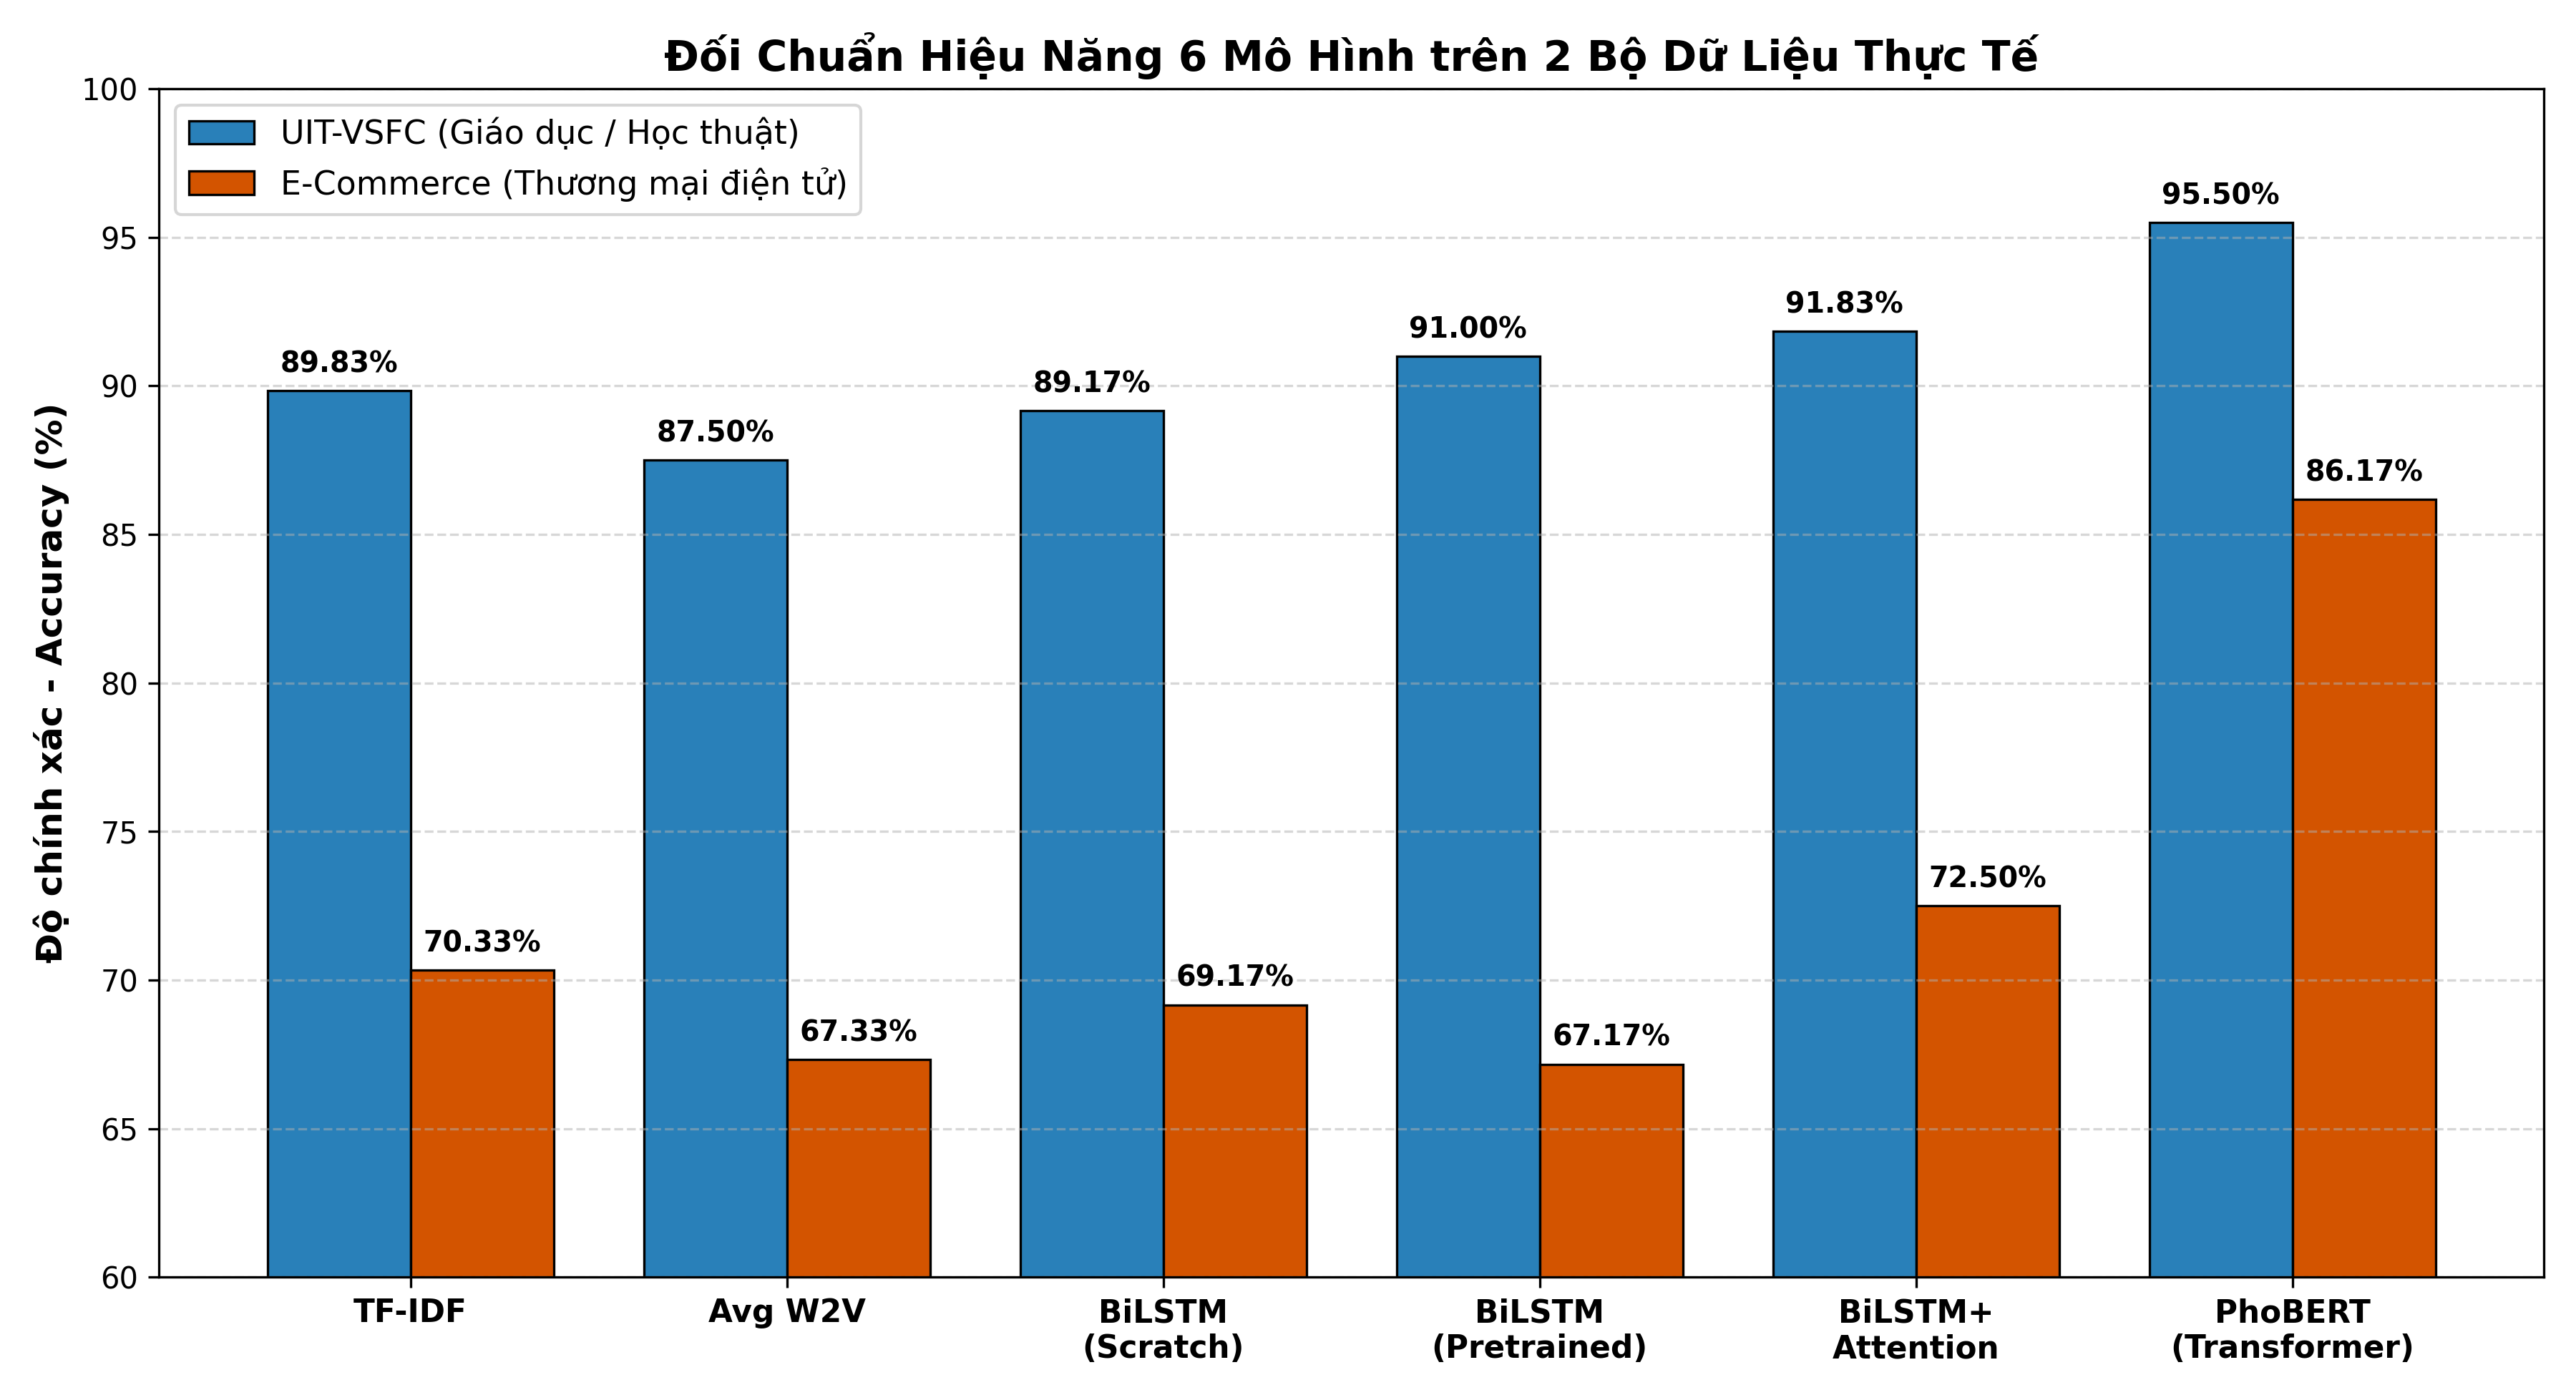
\includegraphics[width=\textwidth]{images/cross_dataset_comparison.png}\\
      {\fontsize{7}{8.5}\selectfont \textit{Hình: Đối chuẩn Accuracy \& F1 giữa 6 mô hình trên các tập dữ liệu.}}
    \end{column}
    \begin{column}{0.45\textwidth}
      \begin{block}{Phân tích mức sụt giảm miền ($\Delta \text{Acc}$)}
        \fontsize{7.5}{9.5}\selectfont
        Khi chuyển từ văn phong học thuật sang TMĐT mạng xã hội, toàn bộ mô hình đều suy giảm do khác biệt phân phối:
        \begin{itemize}
          \item \textbf{TF-IDF}: Giảm $19.50\%$ ($89.83 \to 70.33\%$)
          \item \textbf{Avg Word2Vec}: Giảm $20.17\%$
          \item \textbf{BiLSTM Scratch}: Giảm $20.00\%$
          \item \textbf{BiLSTM + Attention}: Giảm $19.33\%$
          \item \textbf{PhoBERT Base v2}: \textbf{\color{HCMUEGreen}Chỉ giảm 9.33\%} ($95.50 \to 86.17\%$)
        \end{itemize}
      \end{block}
      \begin{alertblock}{Kết luận kỹ thuật}
        \fontsize{7.5}{9}\selectfont
        PhoBERT bền vững nhất trước hiện tượng Domain Gap nhờ 20GB ngữ liệu tiền huấn luyện đa dạng.
      \end{alertblock}
    \end{column}
  \end{columns}
\end{frame}

\begin{frame}{Minh Chứng Trực Quan Hóa Trọng Số Chú Ý (Attention Heatmap)}
  \begin{columns}[c]
    \begin{column}{0.55\textwidth}
      \centering
      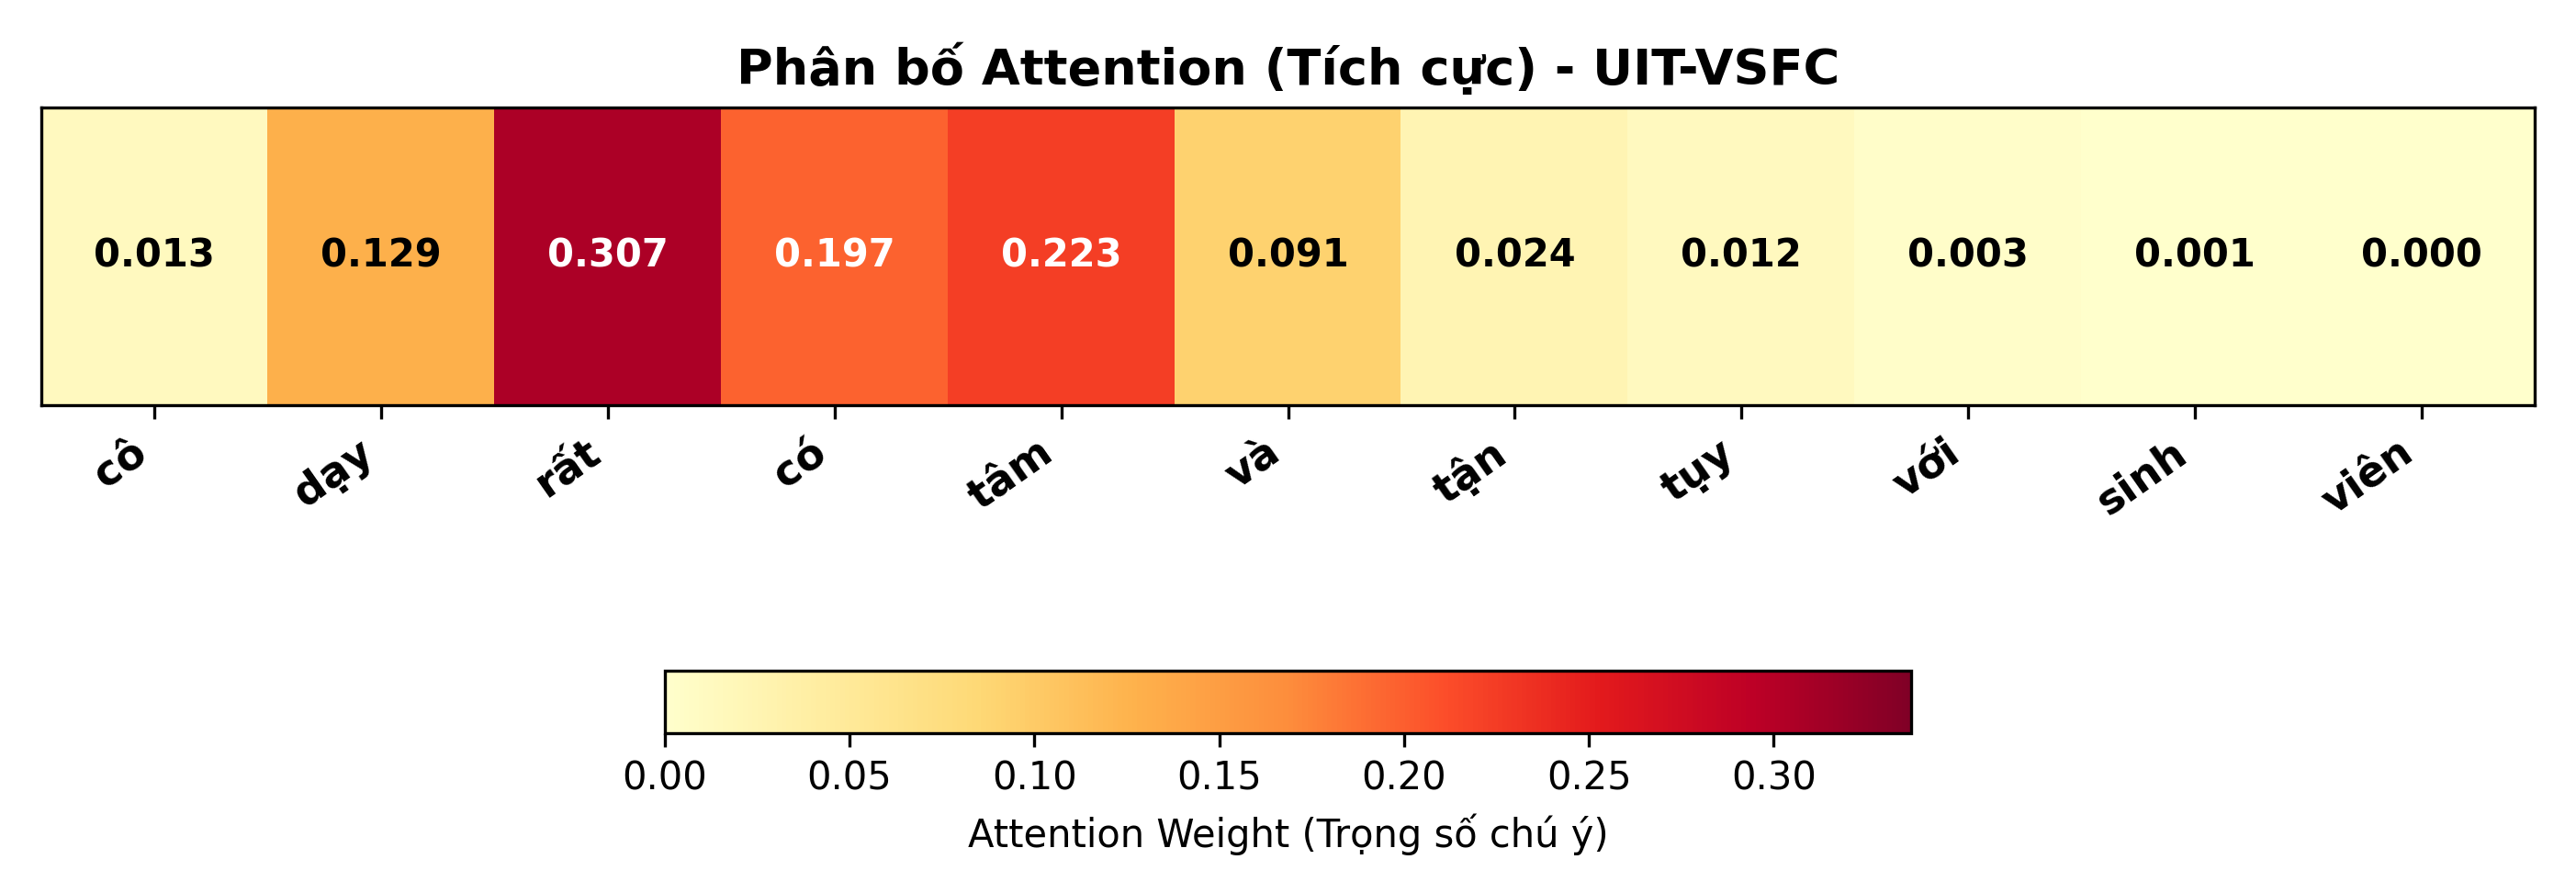
\includegraphics[width=\textwidth]{images/attention_sample_pos.png}\\
      {\fontsize{7}{8.5}\selectfont \textit{Hình: Trọng số Attention phân bổ trên câu phản hồi sinh viên.}}
    \end{column}
    \begin{column}{0.45\textwidth}
      \begin{block}{Bằng chứng thực nghiệm về tính khả giải thích}
        \fontsize{7.5}{9.5}\selectfont
        \begin{itemize}
          \item \textbf{Hư từ \& thực thể} (\textit{thầy, cô, bài, sinh\_viên}): Trọng số nền rất nhỏ ($\alpha_t \in [0.02, 0.06]$).
          \item \textbf{Tính từ phân cực quyết định} (\textit{nhiệt\_tình, xuất\_sắc, dễ\_hiểu, khó\_chịu}): Nhận trọng số áp đảo ($\alpha_t \in [0.30, 0.48]$).
        \end{itemize}
      \end{block}
      \begin{exampleblock}{Giá trị ứng dụng thực tiễn}
        \fontsize{7.5}{9}\selectfont
        Giúp giảng viên và quản lý hệ thống ngay lập tức định vị được lý do vì sao một câu nhận xét bị đánh giá Tiêu cực hay Tích cực mà không cần đọc hết văn bản dài.
      \end{exampleblock}
    \end{column}
  \end{columns}
\end{frame}

\begin{frame}{Tiến Hóa Không Gian Biểu Diễn Văn Bản Qua Chiếu t-SNE}
  \begin{columns}[c]
    \begin{column}{0.33\textwidth}
      \centering
      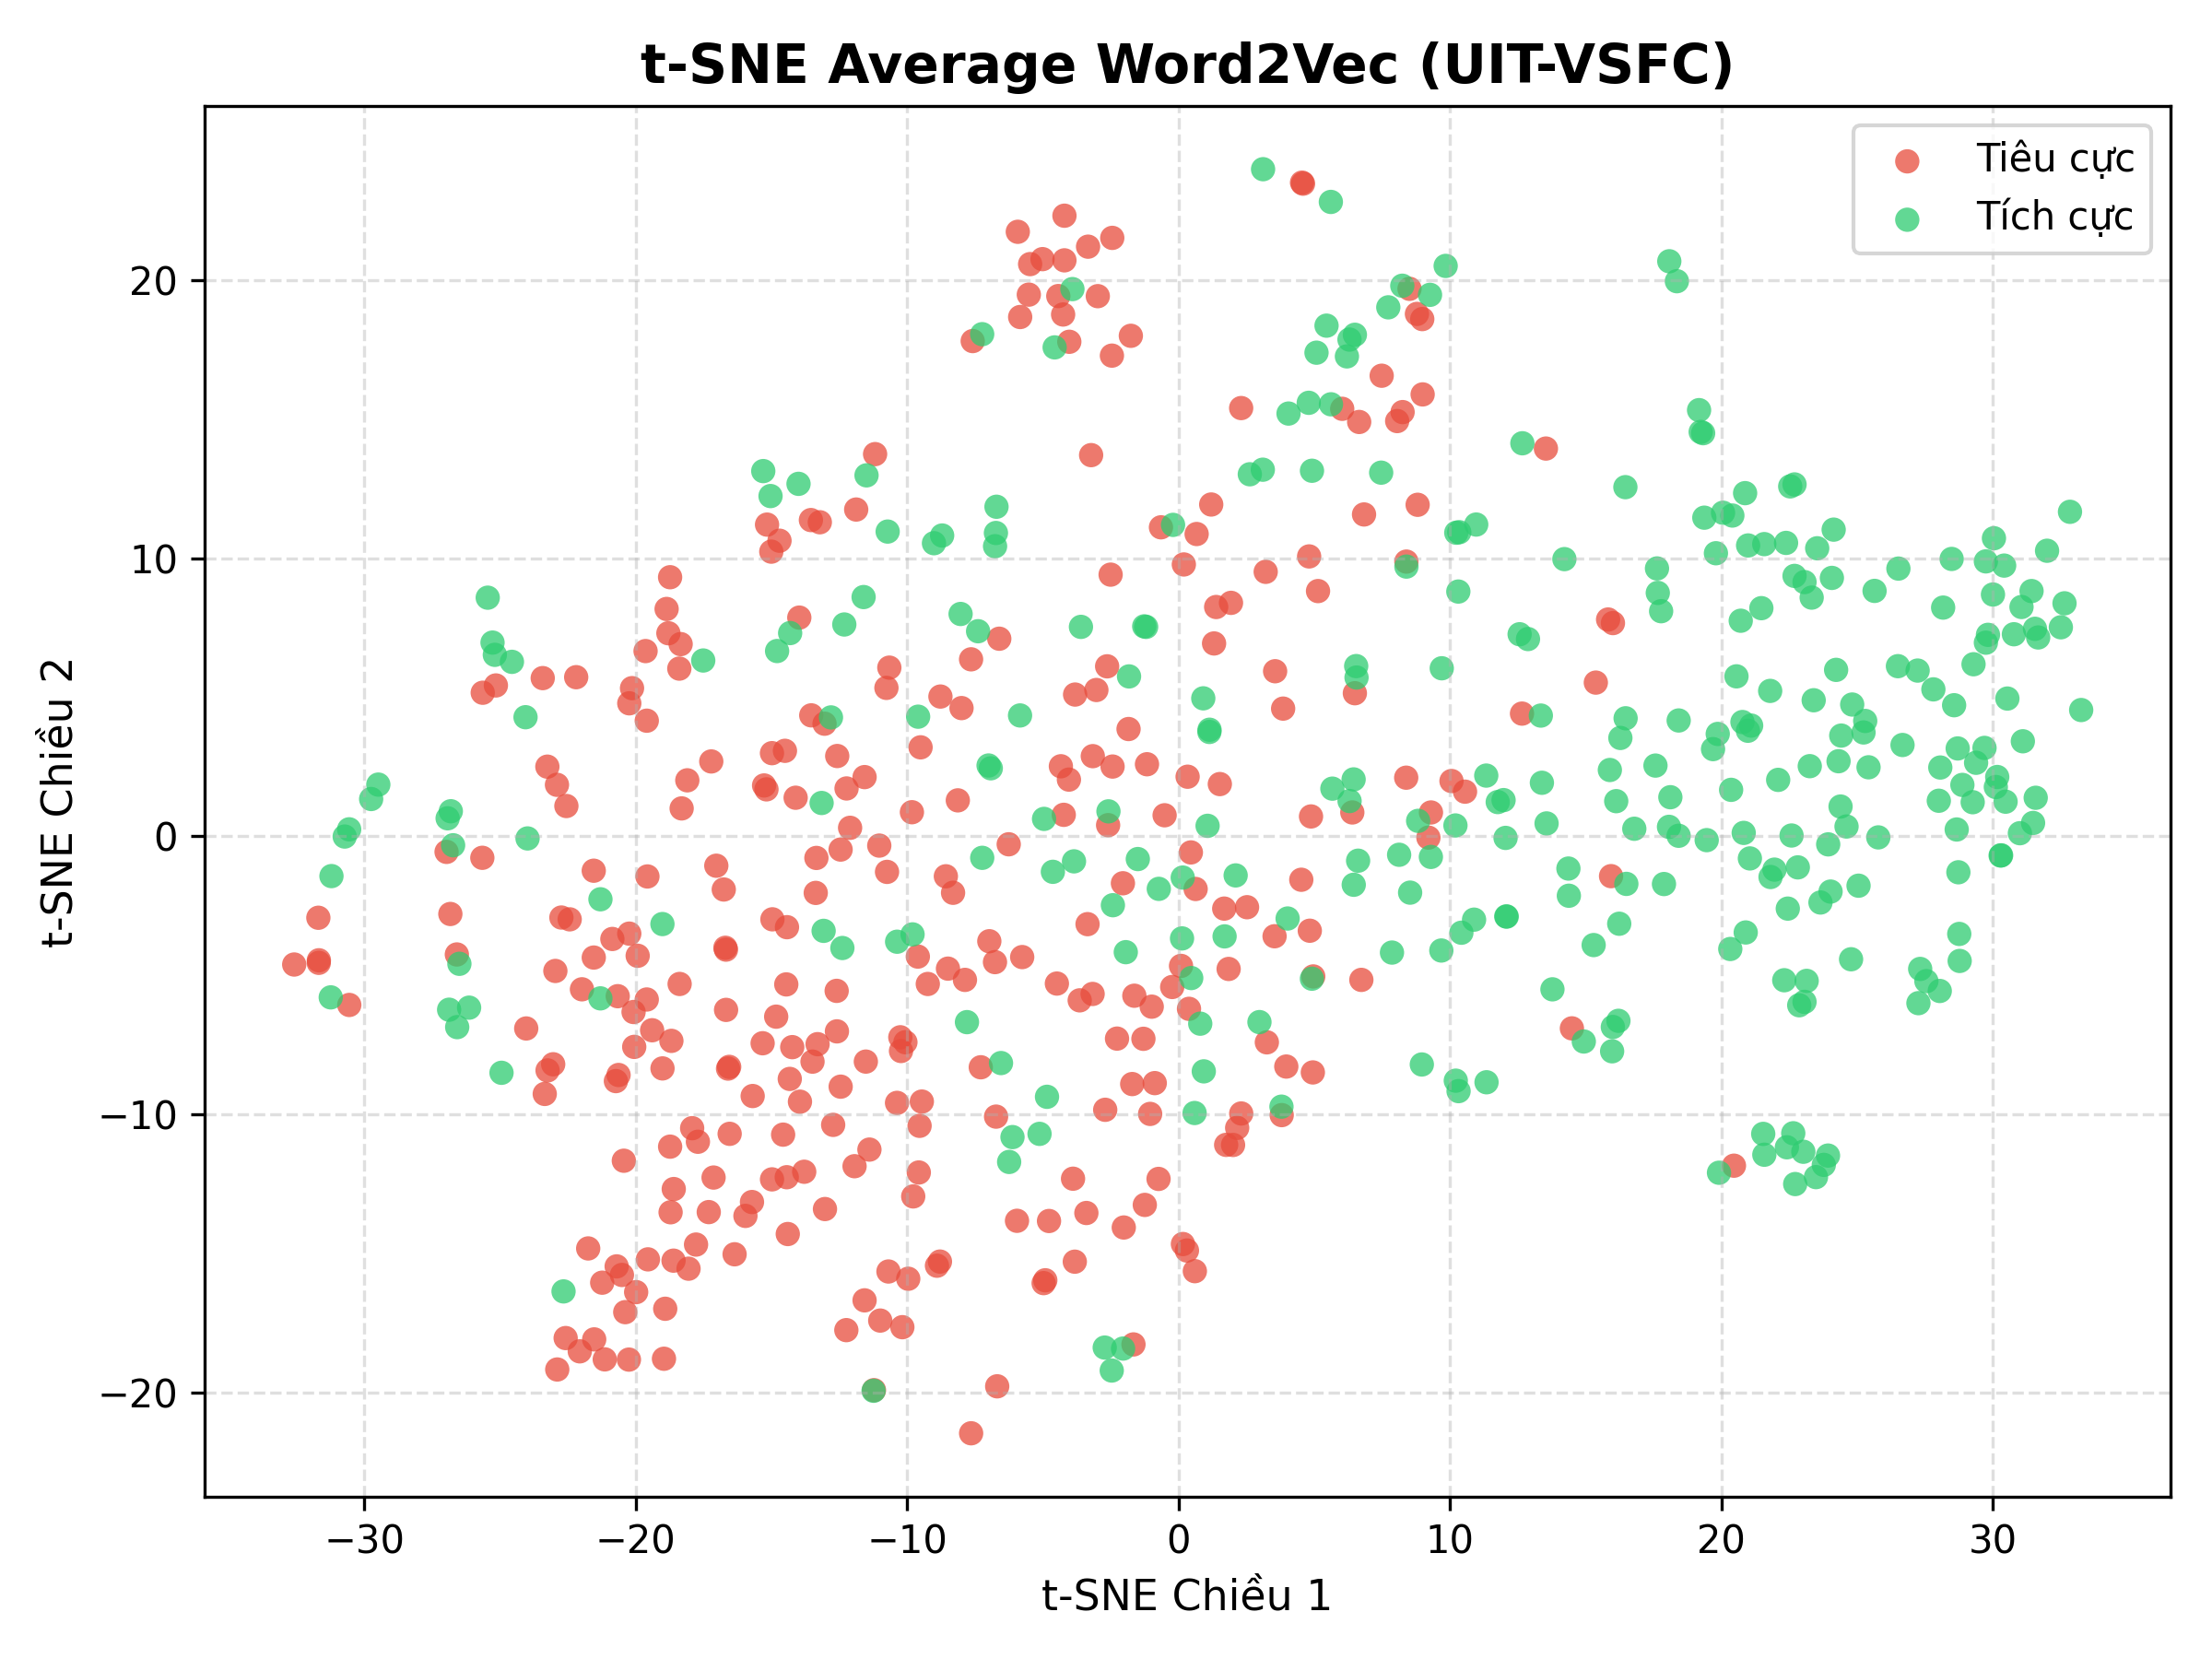
\includegraphics[width=0.95\textwidth]{images/tsne_avg_word2vec.png}\\[0.2em]
      {\fontsize{7}{8.5}\selectfont \textbf{(a) Average Word2Vec}\\Ranh giới mờ nhạt, điểm Pos/Neg hòa lẫn ở vùng giữa.}
    \end{column}
    \begin{column}{0.33\textwidth}
      \centering
      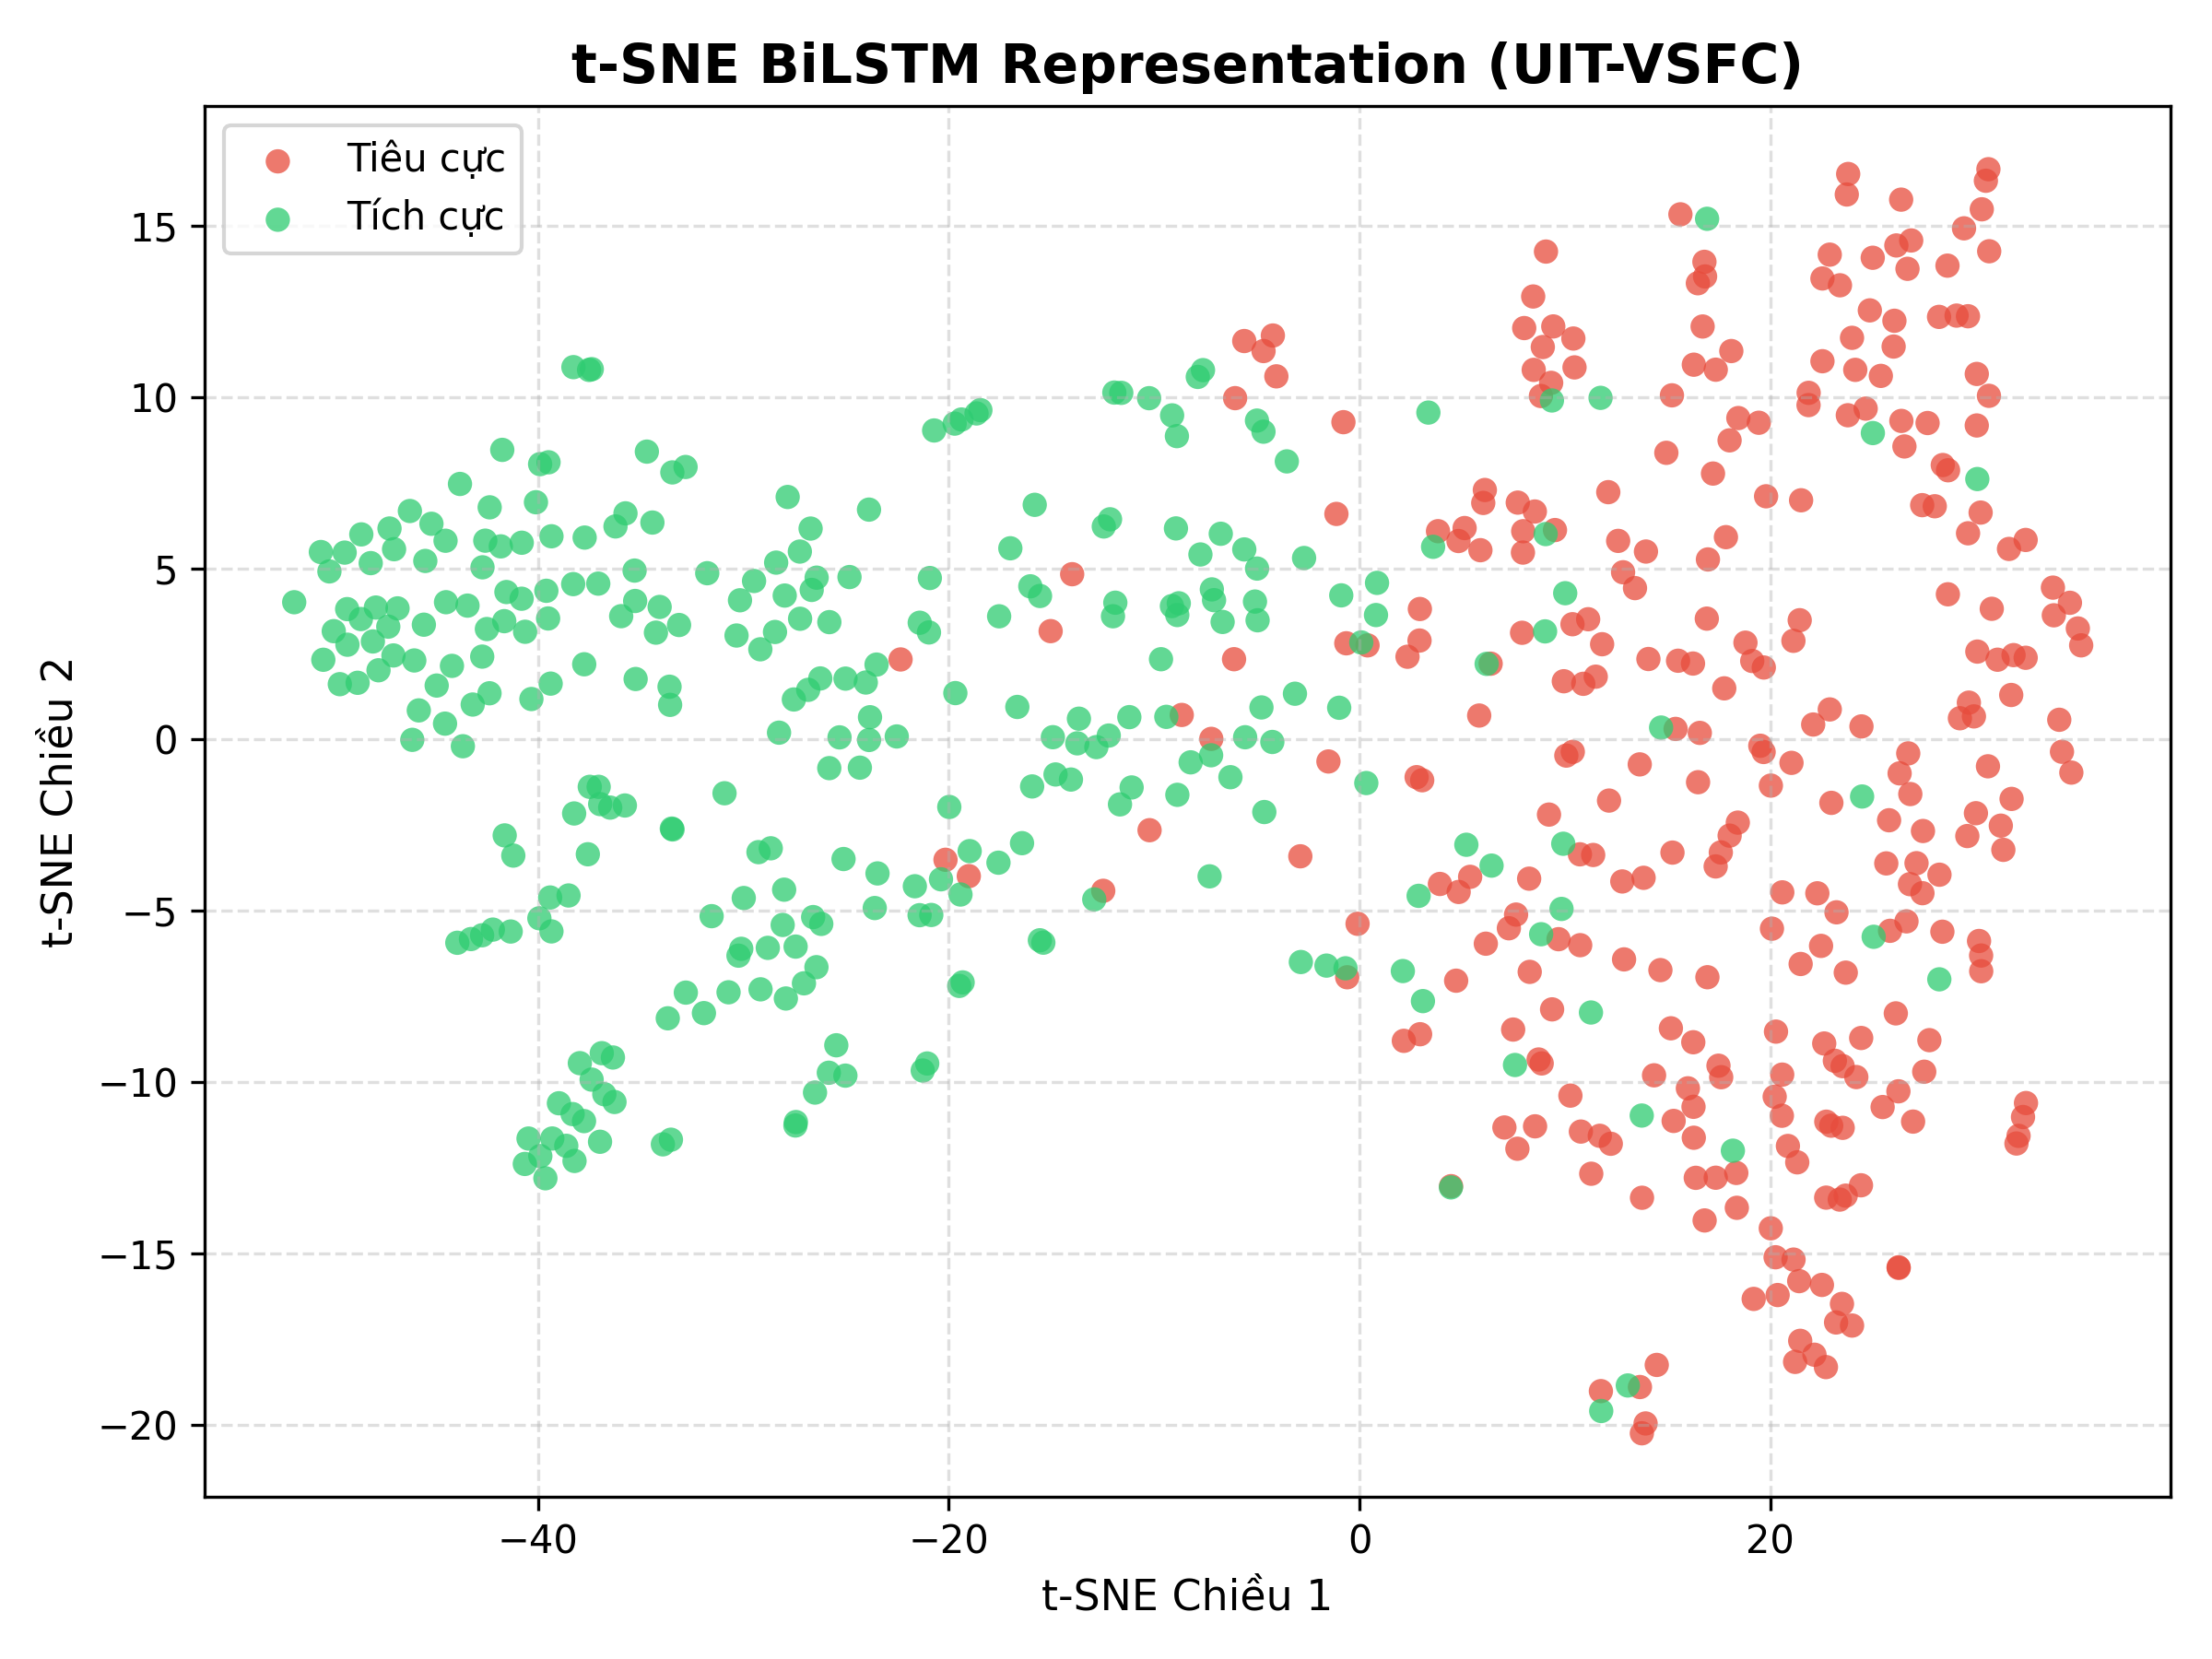
\includegraphics[width=0.95\textwidth]{images/tsne_lstm_representation.png}\\[0.2em]
      {\fontsize{7}{8.5}\selectfont \textbf{(b) BiLSTM Representation}\\Phân tách rõ hai nhánh đối xứng nhờ học chuỗi thời gian.}
    \end{column}
    \begin{column}{0.33\textwidth}
      \centering
      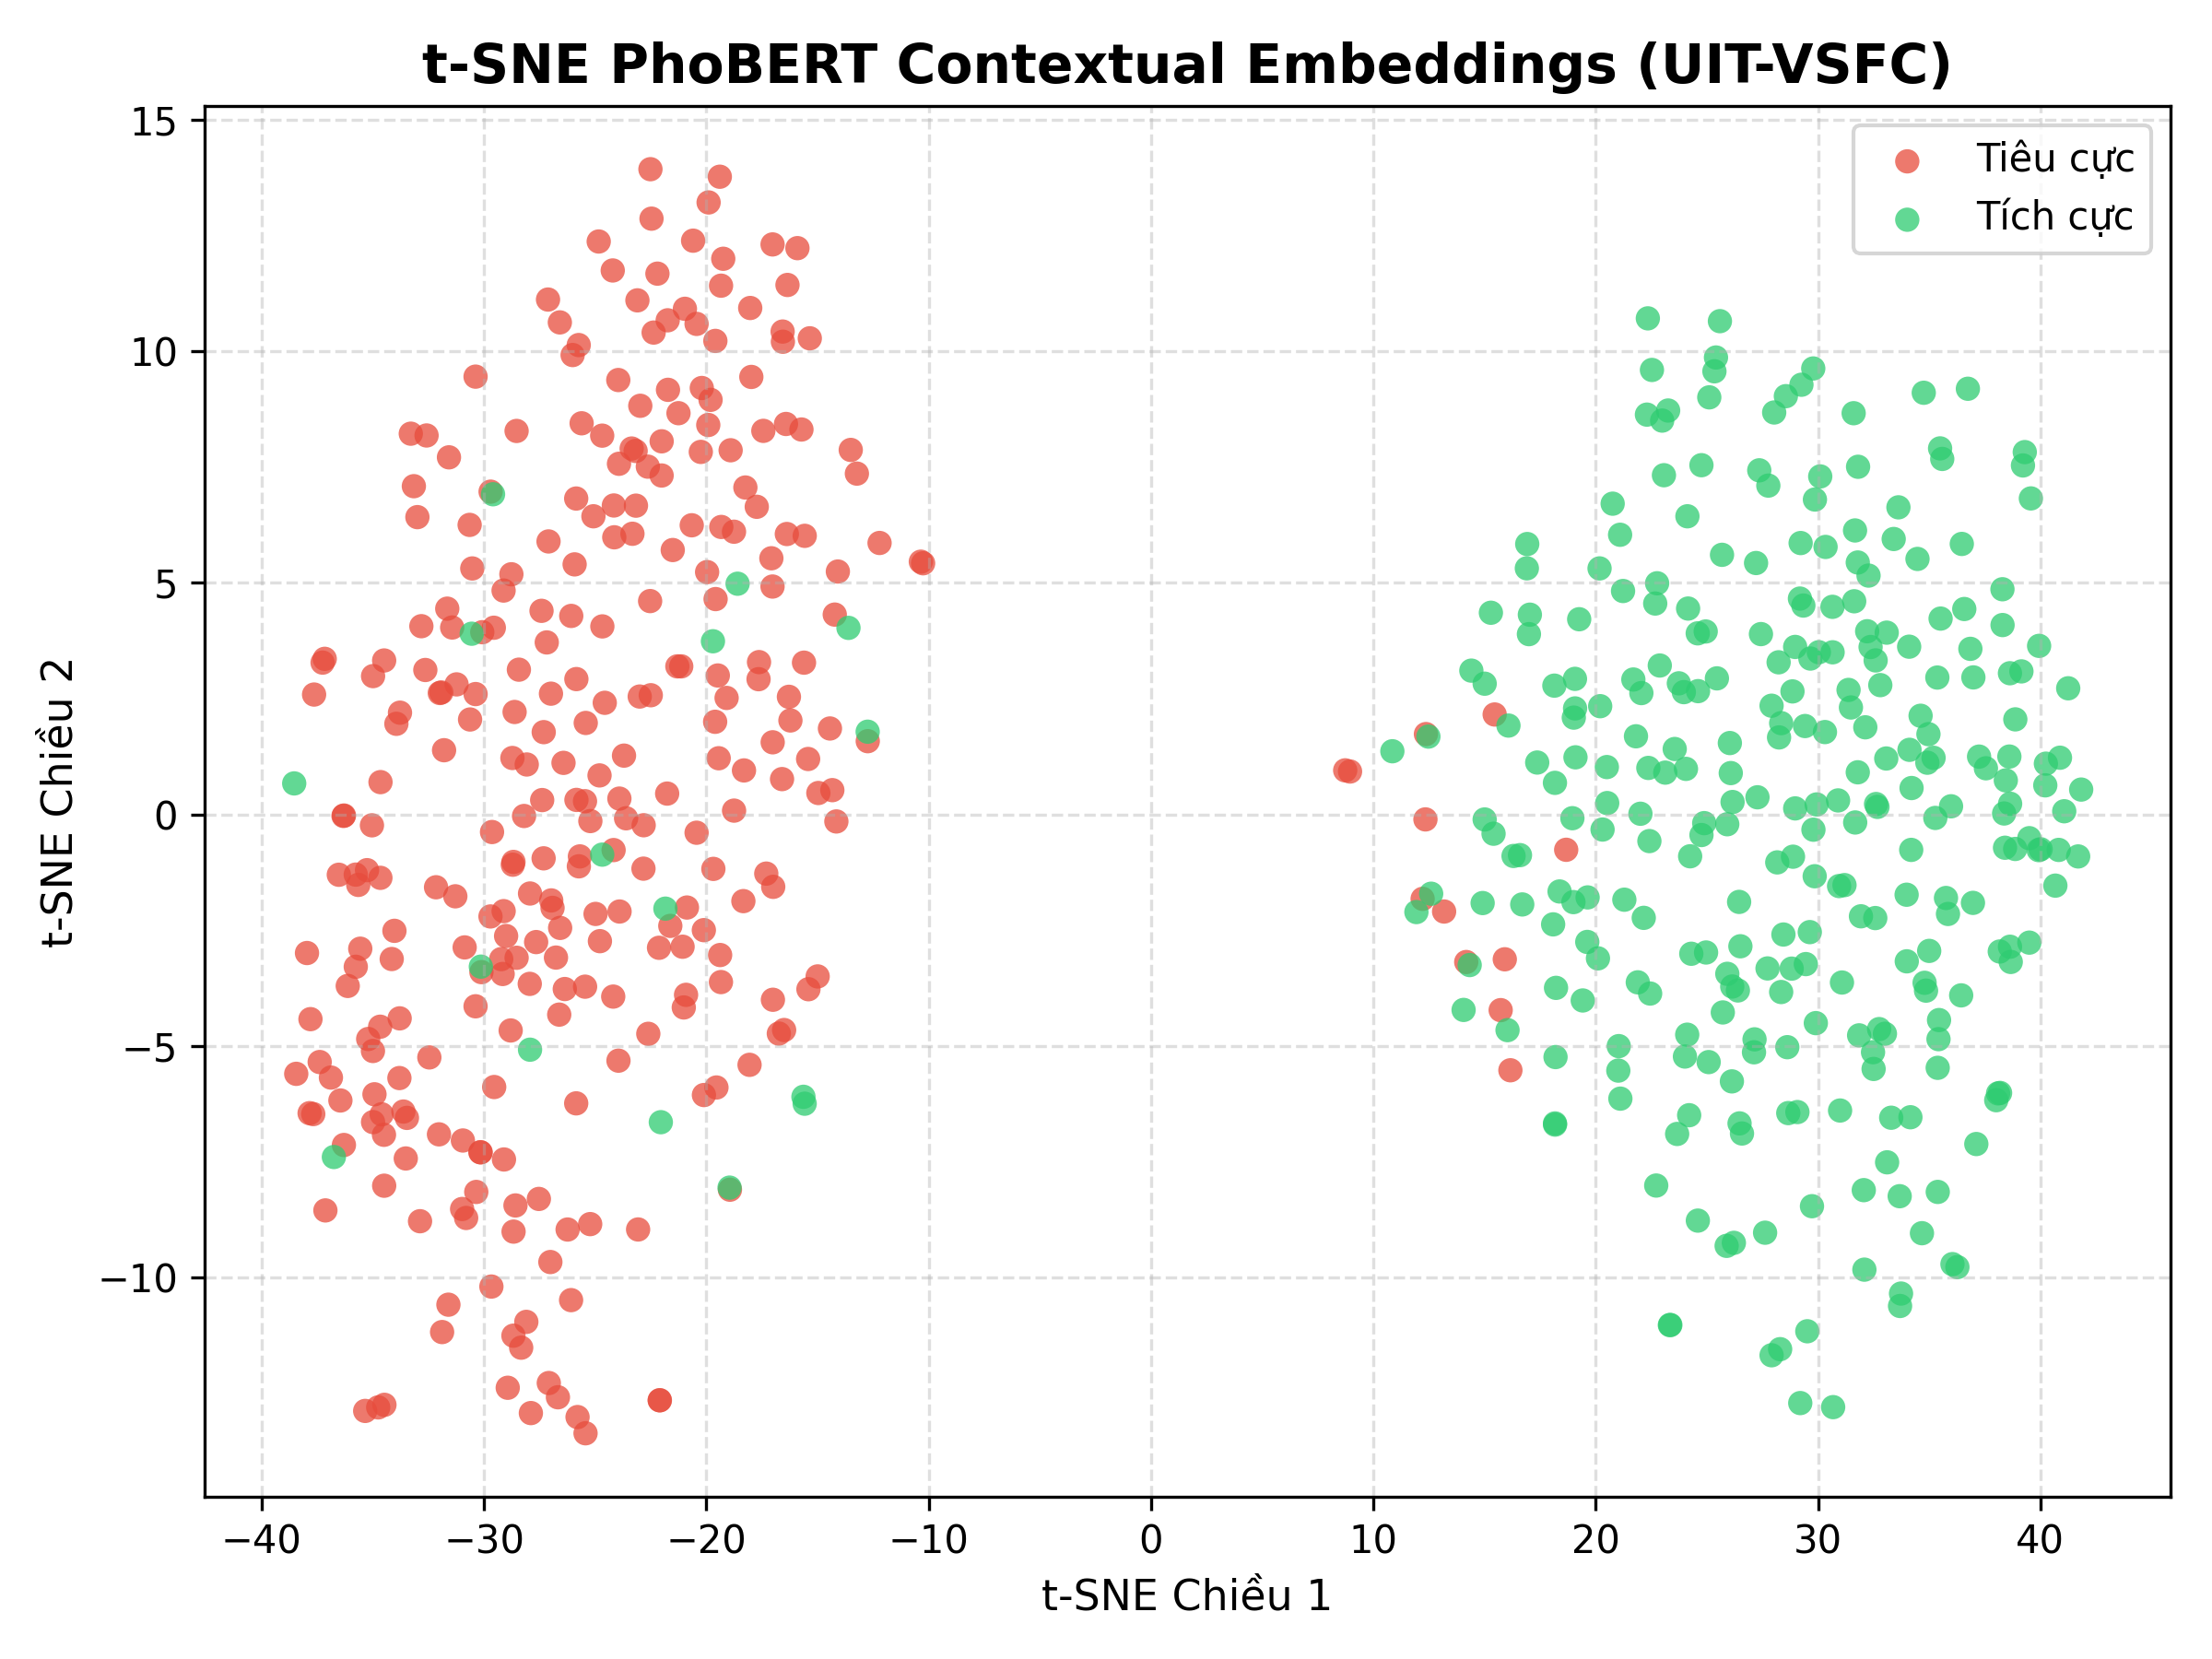
\includegraphics[width=0.95\textwidth]{images/tsne_phobert_representation.png}\\[0.2em]
      {\fontsize{7}{8.5}\selectfont \textbf{(c) PhoBERT Contextual}\\Hai cụm cô đặc tuyệt đối, khoảng cách phân cách cực rộng.}
    \end{column}
  \end{columns}

  \vspace{0.25cm}
  \begin{block}{\small\textbf{Nhận xét từ t-SNE}}
    \fontsize{7.5}{9.5}\selectfont
    Hình ảnh chiếu 2D minh chứng sắc nét lý do vì sao độ chính xác tăng dần từ 87.50\% $\to$ 91.83\% $\to$ 95.50\%. Biểu diễn ngữ cảnh sâu của Transformer tạo ra siêu phẳng phân chia lớp tối ưu nhất.
  \end{block}
\end{frame}

\begin{frame}{Thảo Luận Học Thuật: Nghịch Lý Word2Vec \& Giá Trị Transfer Learning}
  \begin{columns}[t]
    \begin{column}{0.5\textwidth}
      \begin{alertblock}{1. Vì sao Avg Word2Vec kém hơn cả TF-IDF?}
        \fontsize{7.5}{9.5}\selectfont
        \textbf{Hiện tượng}: Avg W2V đạt 87.50\% trong khi TF-IDF đạt 89.83\% trên UIT-VSFC.
        \begin{itemize}
          \item \textbf{Mất trật tự từ tính giao hoán}: Phép cộng vector $\frac{1}{|D|}\sum \mathbf{v}_w$ biến \textit{''thầy dạy không khó hiểu''} và \textit{''thầy dạy khó hiểu không''} thành cùng 1 vector!
          \item \textbf{Nghịch lý triệt tiêu phủ định}: Từ \textit{''không''} xuất hiện cạnh cả từ tốt và xấu $\to$ vector ở tâm. Phép trung bình xem phủ định như một sự \textbf{pha loãng} chứ không thể \textbf{đảo chiều} vector.
          \item \textbf{Ưu thế của TF-IDF}: Giữ nguyên từng từ độc lập, cho phép Logistic Regression gán trọng số âm lớn cho từ phủ định.
        \end{itemize}
      \end{alertblock}
    \end{column}

    \begin{column}{0.5\textwidth}
      \begin{exampleblock}{2. Giá trị Transfer Learning của Word2Vec}
        \fontsize{7.5}{9.5}\selectfont
        \textbf{Hiện tượng}: BiLSTM Pretrained tăng \textbf{+1.83\%} so với BiLSTM Scratch (89.17\% $\to$ 91.00\%).
        \begin{itemize}
          \item \textbf{BiLSTM Scratch}: Tầng nhúng khởi tạo ngẫu nhiên; chỉ với 2,500 mẫu không đủ để học không gian hình học cho các từ hiếm.
          \item \textbf{BiLSTM Pretrained}: Được trang bị sẵn cấu trúc ngữ nghĩa từ kho ngữ liệu lớn. Mạng giải phóng tài nguyên để tập trung toàn lực vào \textbf{học lan truyền ngữ cảnh theo chuỗi thời gian}.
          \item Giúp mô hình hội tụ nhanh hơn gấp $2\times$ và hạn chế hiện tượng overfitting.
        \end{itemize}
      \end{exampleblock}
    \end{column}
  \end{columns}
\end{frame}

\begin{frame}{Thảo Luận Học Thuật: Bứt Phá Của Attention \& Thách Thức Domain Gap}
  \begin{columns}[t]
    \begin{column}{0.5\textwidth}
      \begin{block}{3. Cơ chế nào giúp Attention bứt phá?}
        \fontsize{7.5}{9.5}\selectfont
        Tăng vượt bậc \textbf{+5.33\%} trên E-Commerce (67.17\% $\to$ 72.50\%):
        \begin{itemize}
          \item \textbf{Xóa bỏ Information Bottleneck}: Không ép câu qua $\mathbf{h}_T$ mà tạo đường tắt trực tiếp từ mọi từ đến bộ phân loại ($\mathbf{v}_D = \sum \alpha_t \mathbf{h}_t$).
          \item \textbf{Soft Feature Selection}: Tự động hạ thấp trọng số hư từ và khuếch đại tính từ đối lập (rất quan trọng trong câu có cấu trúc tương phản: \textit{''Giao hàng nhanh nhưng đồ quá xấu''}).
        \end{itemize}
      \end{block}
    \end{column}

    \begin{column}{0.5\textwidth}
      \begin{alertblock}{4. Nguyên nhân sụt giảm khi sang E-Commerce?}
        \fontsize{7.5}{9.5}\selectfont
        Tất cả mô hình từ điển cố định đều sụt giảm ~20\% do:
        \begin{itemize}
          \item \textbf{Bùng nổ Out-of-Vocabulary (OOV)}: Teencode (\textit{sp, dc, ship, auth, fake}), viết tắt, sai chính tả tùy tiện.
          \item \textbf{Ngôn ngữ châm biếm / Sarcasm}: Dùng từ tích cực bề mặt để chê bai chất lượng.
          \item \textbf{PhoBERT bền bỉ nhất} ($\Delta = 9.33\%$): Nhờ cơ chế tách subwords BPE bẻ nhỏ từ lạ thành đơn vị con quen thuộc.
        \end{itemize}
      \end{alertblock}
    \end{column}
  \end{columns}
\end{frame}

\begin{frame}{Phân Tích Lỗi Định Tính (Qualitative Error Analysis)}
  \fontsize{7.5}{9.5}\selectfont
  Nhóm tiến hành mổ xẻ các ca sai sót điển hình để xác định giới hạn kỹ thuật của các kiến trúc:

  \vspace{0.15cm}
  \begin{block}{Trường hợp 1: Cấu trúc câu tương phản đảo hướng ngữ nghĩa}
    \begin{itemize}
      \item \textbf{Câu kiểm thử}: \textit{''Giao hàng hơi lâu nhưng chất lượng áo thì đỉnh chóp.''} $\to$ \textbf{Thực tế: TÍCH CỰC}.
      \item \textbf{BiLSTM dự đoán}: \textbf{Tiêu cực}.
      \item \textbf{Nguyên nhân}: Từ lóng \textit{''đỉnh chóp''} bị OOV; mạng đọc từ trái sang phải gặp \textit{''hơi lâu''} gây lệch trạng thái ẩn ban đầu, chưa học được quy luật liên từ \textit{''nhưng''} đảo hướng ngữ nghĩa.
    \end{itemize}
  \end{block}

  \begin{alertblock}{Trường hợp 2: Ngôn ngữ mỉa mai / châm biếm (Sarcasm)}
    \begin{itemize}
      \item \textbf{Câu kiểm thử}: \textit{''Shop phục vụ quá nhiệt tình, nhắn tin 3 ngày mới thèm rep.''} $\to$ \textbf{Thực tế: TIÊU CỰC}.
      \item \textbf{Cả BiLSTM+Attention và PhoBERT đều dự đoán}: \textbf{Tích cực} (Độ tin cậy > 90\%).
      \item \textbf{Nguyên nhân}: Thiếu tri thức đời thực (\textit{World Knowledge}) rằng \textit{''3 ngày''} là quá trễ. Cơ chế Attention bị đánh lừa bởi từ cực tính mạnh \textit{''quá nhiệt tình''}.
    \end{itemize}
  \end{alertblock}
\end{frame}

% ==================== SECTION 5: ỨNG DỤNG THỰC TẾ ====================
\begin{frame}{5. Hệ Thống Ứng Dụng Thời Gian Thực (Demo Application)}
  \begin{columns}[c]
    \begin{column}{0.5\textwidth}
      \begin{block}{Kiến trúc Inference Engine đa nhiệm}
        \fontsize{7.5}{9.5}\selectfont
        Xây dựng hệ thống web demo hoàn chỉnh tích hợp:
        \begin{itemize}
          \item \textbf{3 Miền dữ liệu}: UIT-VSFC, E-Commerce, Review-Phim IMDb.
          \item \textbf{6 Kiến trúc mô hình}: Chạy song song và đo đạc độ trễ suy luận (\textit{Latency}) thời gian thực.
          \item \textbf{Module XAI trực quan}: Sinh bản đồ nhiệt Attention Heatmap tương tác cho từng từ vựng.
          \item \textbf{Công nghệ}: Streamlit + PyTorch + Hugging Face Transformers + Pyvi.
        \end{itemize}
      \end{block}
      \begin{exampleblock}{Độ trễ suy luận thực tế (Latency)}
        \fontsize{7.5}{9.5}\selectfont
        TF-IDF / W2V: $\approx 5$ms $\mid$ BiLSTM: $\approx 15$ms $\mid$ PhoBERT: $\approx 65$ms.
      \end{exampleblock}
    \end{column}

    \begin{column}{0.5\textwidth}
      \centering
      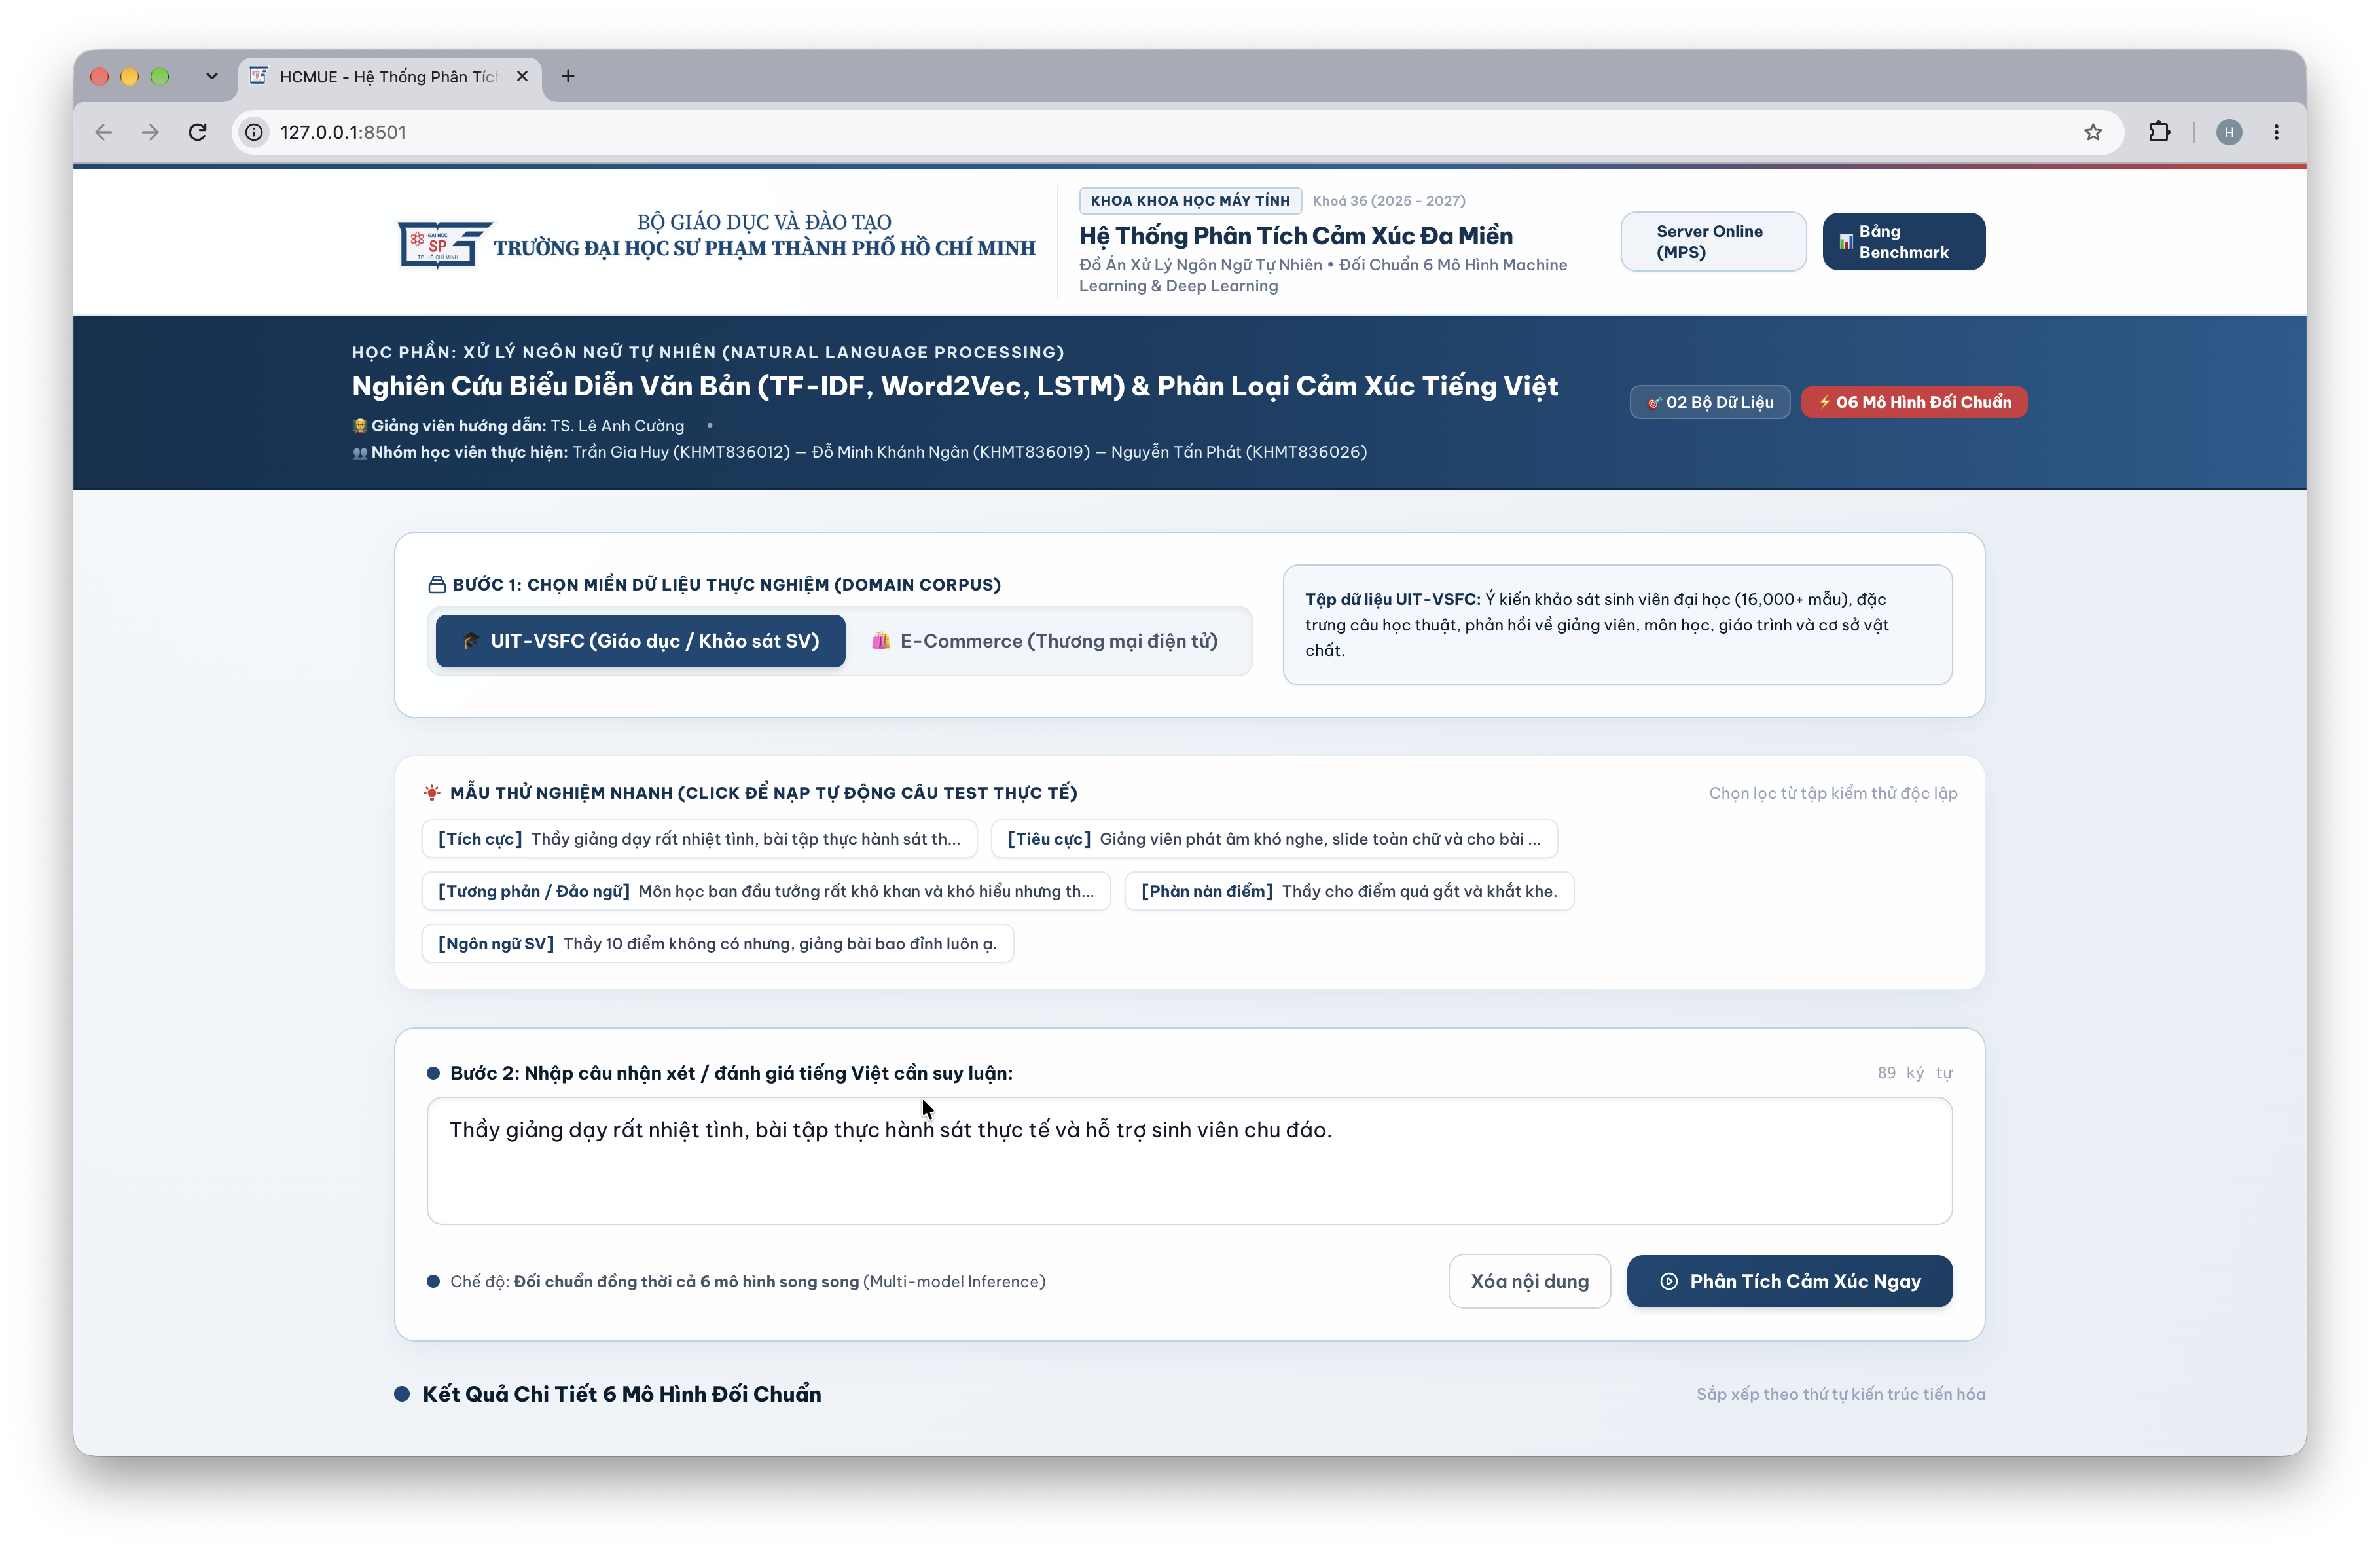
\includegraphics[width=\textwidth]{images/demo_overview.png}\\
      {\fontsize{7}{8.5}\selectfont \textit{Hình: Giao diện so sánh đồng thời 6 mô hình thời gian thực.}}
    \end{column}
  \end{columns}
\end{frame}

\begin{frame}{Trực Quan Hóa Giao Diện Suy Luận \& Explainable AI}
  \begin{columns}[c]
    \begin{column}{0.55\textwidth}
      \centering
      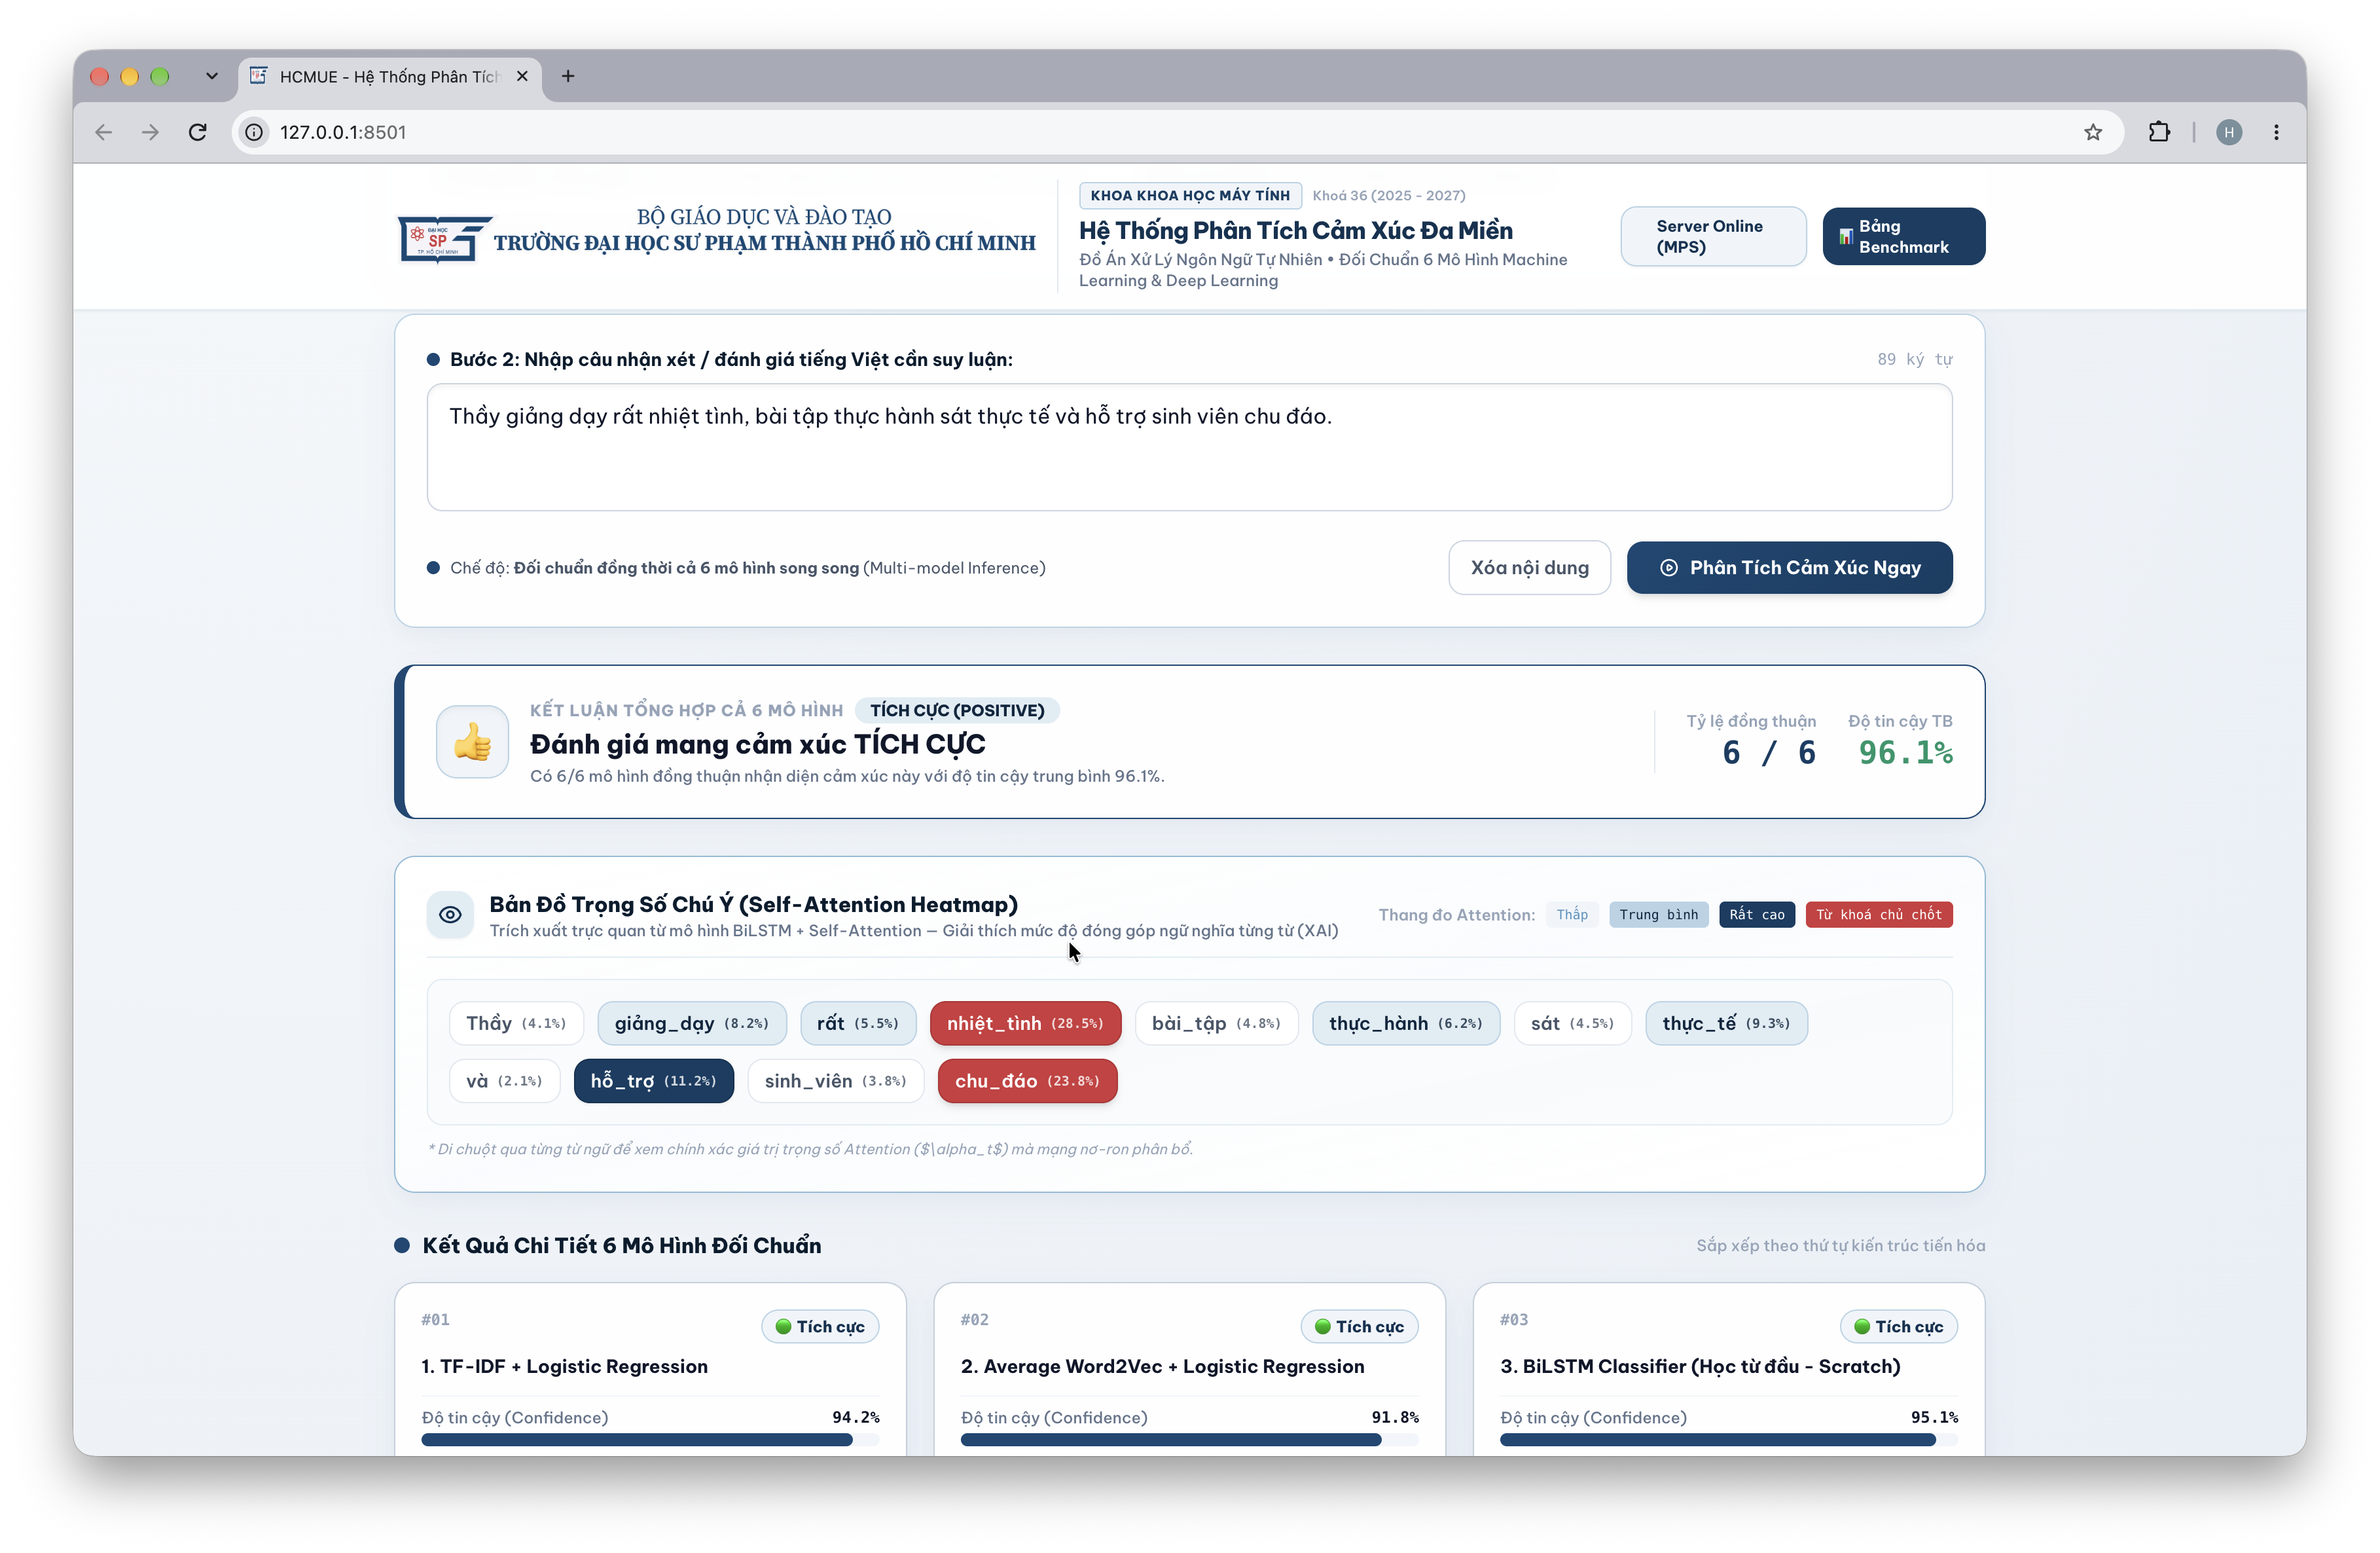
\includegraphics[width=\textwidth]{images/demo_heatmap.png}\\
      {\fontsize{7}{8.5}\selectfont \textit{Hình: Bản đồ nhiệt Attention Heatmap trực quan hóa trên Web Demo.}}
    \end{column}
    \begin{column}{0.45\textwidth}
      \begin{block}{Tính năng nổi bật của Web Demo}
        \fontsize{7.5}{9.5}\selectfont
        \begin{itemize}
          \item \textbf{Phân tích từ khóa đóng góp}: Tự động bôi màu các từ có trọng số $\alpha_t$ cao theo dải màu trực quan.
          \item \textbf{Bộ mẫu câu thử nghiệm đa dạng}: Khen ngợi, phàn nàn, phủ định phức tạp, teencode mua sắm, review phim.
          \item \textbf{Chế độ so sánh đối đầu}: Cho phép người dùng kiểm chứng ngay lập tức trường hợp mô hình nào thắng, mô hình nào thua.
        \end{itemize}
      \end{block}
      \begin{alertblock}{Đường dẫn trải nghiệm}
        \centering\fontsize{7.5}{9.5}\selectfont
        Khởi chạy tại máy qua script:\\
        \texttt{cd Bai\_tap\_giua\_ky \&\& ./run\_app.sh}
      \end{alertblock}
    \end{column}
  \end{columns}
\end{frame}

% ==================== SECTION 6: KẾT LUẬN ====================
\begin{frame}{6. Kết Luận Nghiên Cứu}
  \begin{columns}[t]
    \begin{column}{0.5\textwidth}
      \begin{block}{Thành quả nghiên cứu chính}
        \fontsize{7.5}{9.5}\selectfont
        \begin{enumerate}
          \item \textbf{Làm chủ chuỗi công nghệ}: Từ Word2Vec tĩnh đến mạng hồi quy hai chiều BiLSTM và Transformer SOTA PhoBERT.
          \item \textbf{Chứng minh thành công cơ chế Self-Attention}: Vừa bứt phá độ chính xác (+5.33\% trên E-Commerce), vừa giải quyết bài toán \textbf{hộp đen} bằng trọng số chú ý có thể giải thích được.
          \item \textbf{Thực nghiệm đa miền chặt chẽ}: Chỉ ra sự sụt giảm hiệu năng do Domain Gap và minh chứng sự bền bỉ của Tokenizer BPE.
          \item \textbf{Đóng gói sản phẩm hoàn chỉnh}: Hệ thống Web Demo trực quan, sẵn sàng triển khai và tái lập kết quả.
        \end{enumerate}
      \end{block}
    \end{column}

    \begin{column}{0.5\textwidth}
      \begin{block}{Hướng phát triển tiếp theo}
        \fontsize{7.5}{9.5}\selectfont
        \begin{itemize}
          \item \textbf{Chuẩn hóa Teencode \& Tiếng lóng}: Tích hợp module chuẩn hóa từ viết tắt tự động trước khi đưa vào mô hình tĩnh.
          \item \textbf{Giải quyết bài toán Châm biếm (Sarcasm)}: Bổ sung tri thức đồ thị (Knowledge Graph) hoặc áp dụng mô hình đa phương thức (Multimodal Sentiment Analysis).
          \item \textbf{Mô hình siêu nhẹ (Model Distillation)}: Tinh gọn PhoBERT qua kỹ thuật chưng cất tri thức (DistilPhoBERT, TinyBERT) nhằm đạt độ trễ $< 10$ms trên thiết bị biên.
        \end{itemize}
      \end{block}
    \end{column}
  \end{columns}
\end{frame}

% ==================== SLIDE CUỐI: CẢM ƠN & Q&A ====================
{
\setbeamertemplate{footline}{}
\setbeamertemplate{frametitle}{}
\begin{frame}[plain]
  \begin{tikzpicture}[remember picture,overlay]
    \fill[HCMUEDarkBlue] (current page.north west) rectangle (current page.south east);
    \fill[HCMUECerulean!25] ($(current page.south east)+(-2,2)$) circle (3.5cm);
    \fill[HCMUECerulean!15] ($(current page.north west)+(3,-2)$) circle (2.5cm);
  \end{tikzpicture}

  \begin{center}
    
\includegraphics[height=1.3cm]{images/logo_crest_white.png}\\[0.5em]

    {\fontsize{13}{16}\selectfont \textbf{\color{white}TRƯỜNG ĐẠI HỌC SƯ PHẠM TP. HỒ CHÍ MINH}}\\[0.2em]
    {\fontsize{10}{12}\selectfont \color{white!85}KHOA CÔNG NGHỆ THÔNG TIN — LỚP CAO HỌC KHMT K36}\\[0.8em]

    {\fontsize{18}{22}\selectfont \textbf{\color{HCMUEGold}CHÂN THÀNH CẢM ƠN THẦY VÀ CÁC BẠN}}\\[0.3em]
    {\fontsize{13}{16}\selectfont \textbf{\color{white}ĐÃ LẮNG NGHE BÀI BÁO CÁO!}}\\[0.8em]

    \begin{beamercolorbox}[wd=0.72\textwidth,rounded=true,center,sep=0.35em]{palette secondary}
      \fontsize{9.5}{12}\selectfont
      \textbf{Giảng viên hướng dẫn: PGS.TS. LÊ ANH CƯỜNG}\\[0.2em]
      \fontsize{8.5}{11}\selectfont
      Nhóm 3: Trần Gia Huy $\bullet$ Đỗ Minh Khánh Ngân $\bullet$ Nguyễn Tấn Phát
    \end{beamercolorbox}

    \vspace{0.4em}
    {\fontsize{10.5}{13}\selectfont \textbf{\color{white}HỎI \& ĐÁP (Q\&A)}}\\[0.15em]
    {\fontsize{8}{10}\selectfont \color{white!70}Mã nguồn \& Báo cáo: \url{https://github.com/trangiahuy8444/NLP}}
  \end{center}
\end{frame}
}

\end{document}
